\begin{figure}
  \centering
  \begin{subfigure}[b]{0.47\linewidth}
      \centering
      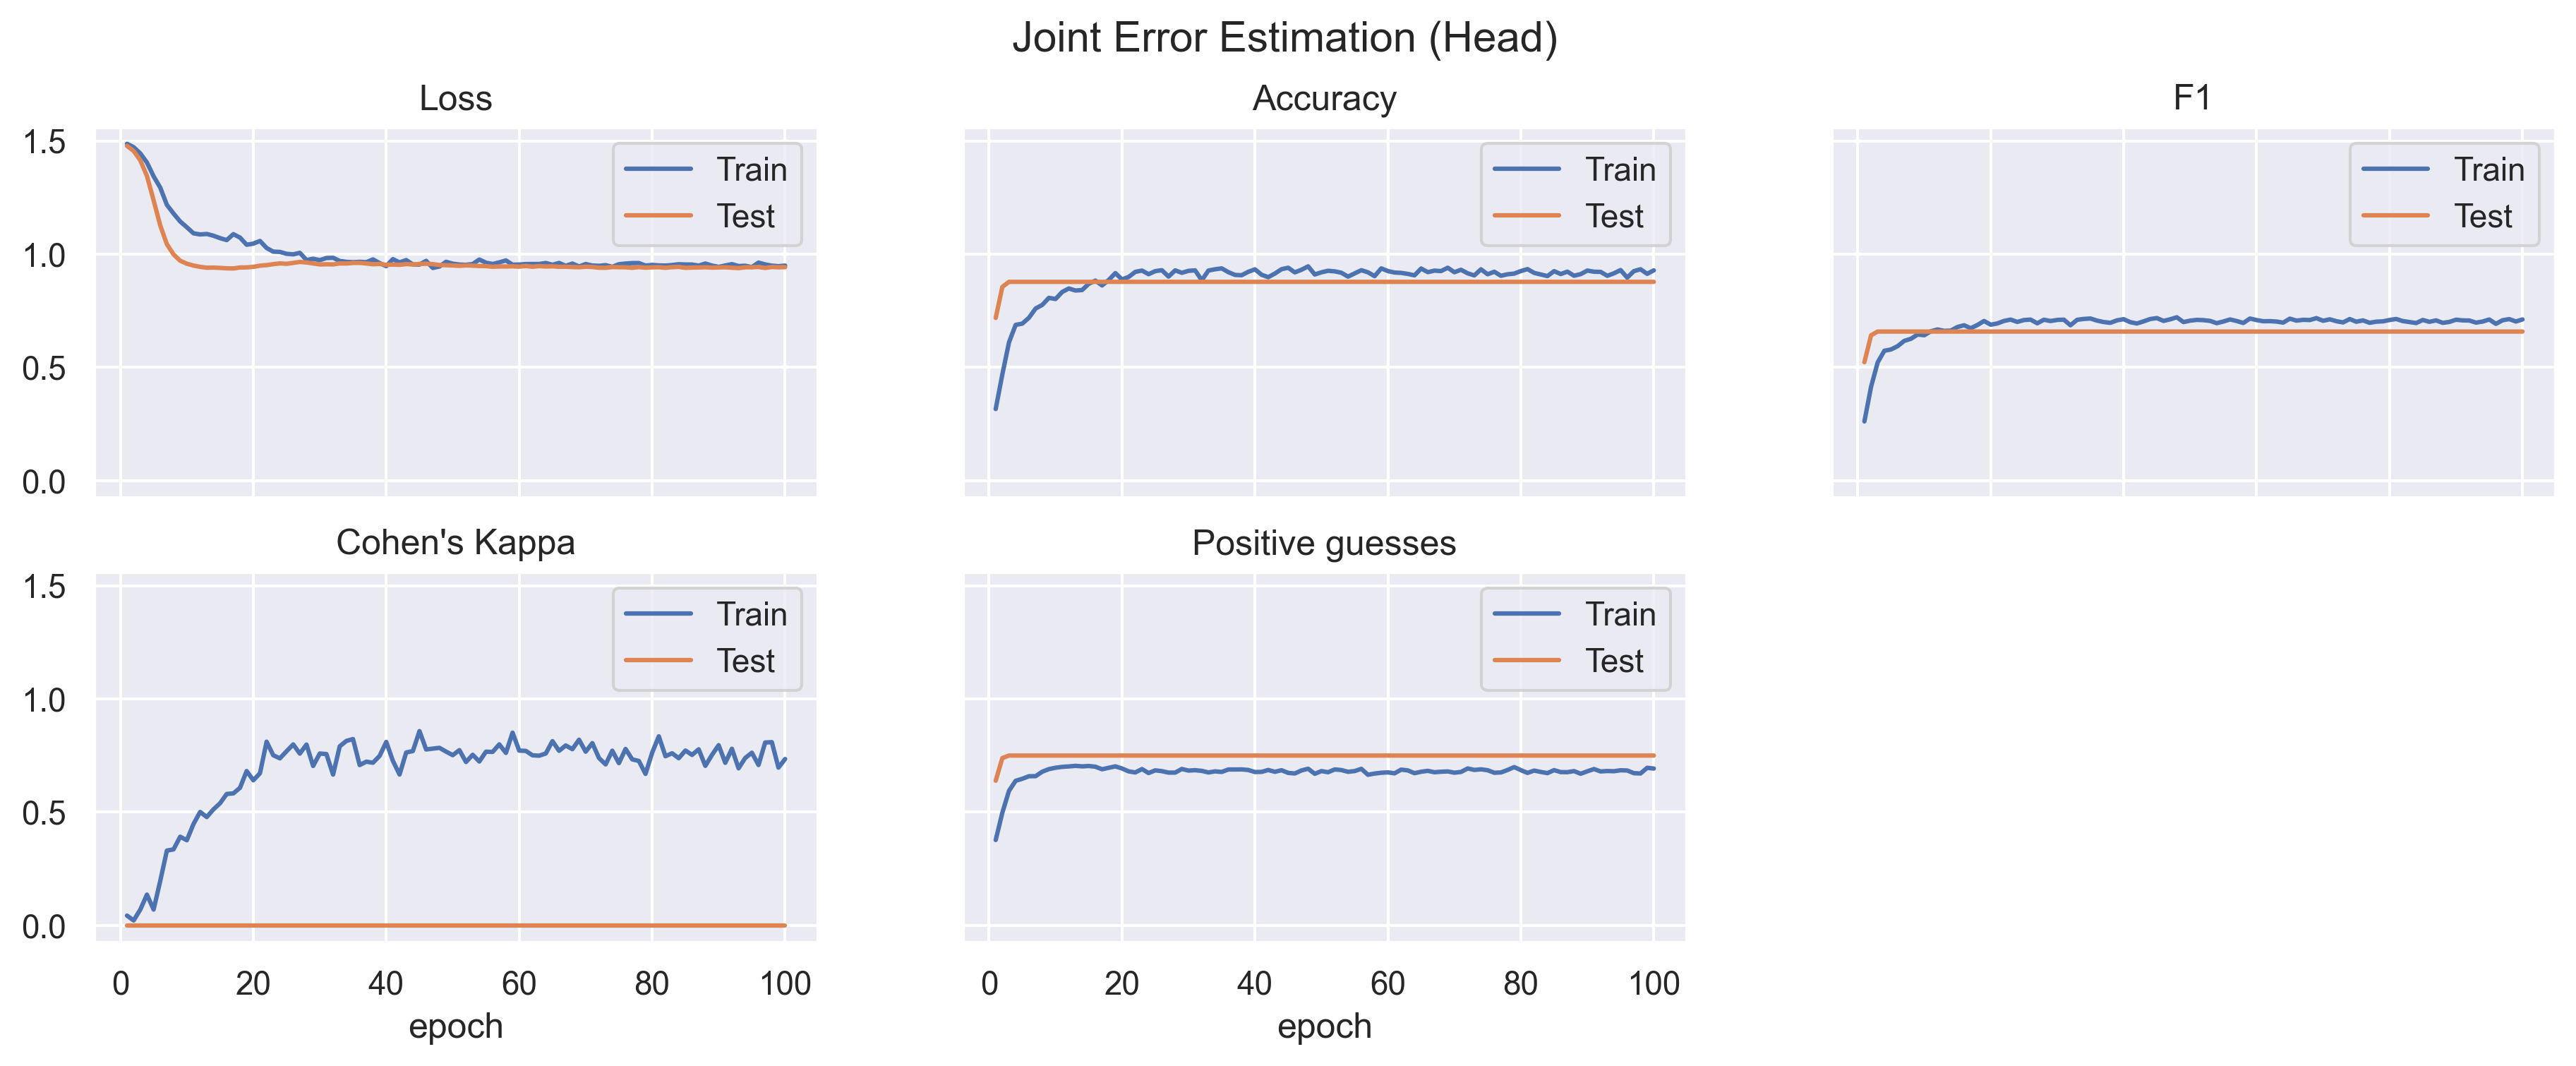
\includegraphics[width=\textwidth]{figures/Results/jt/JointErrorEstimation_Head.png}
      \caption{Head Error Estimation}
      \label{fig:head_jt_ee}
  \end{subfigure}
  \hfill
  \begin{subfigure}[b]{0.47\linewidth}
      \centering
      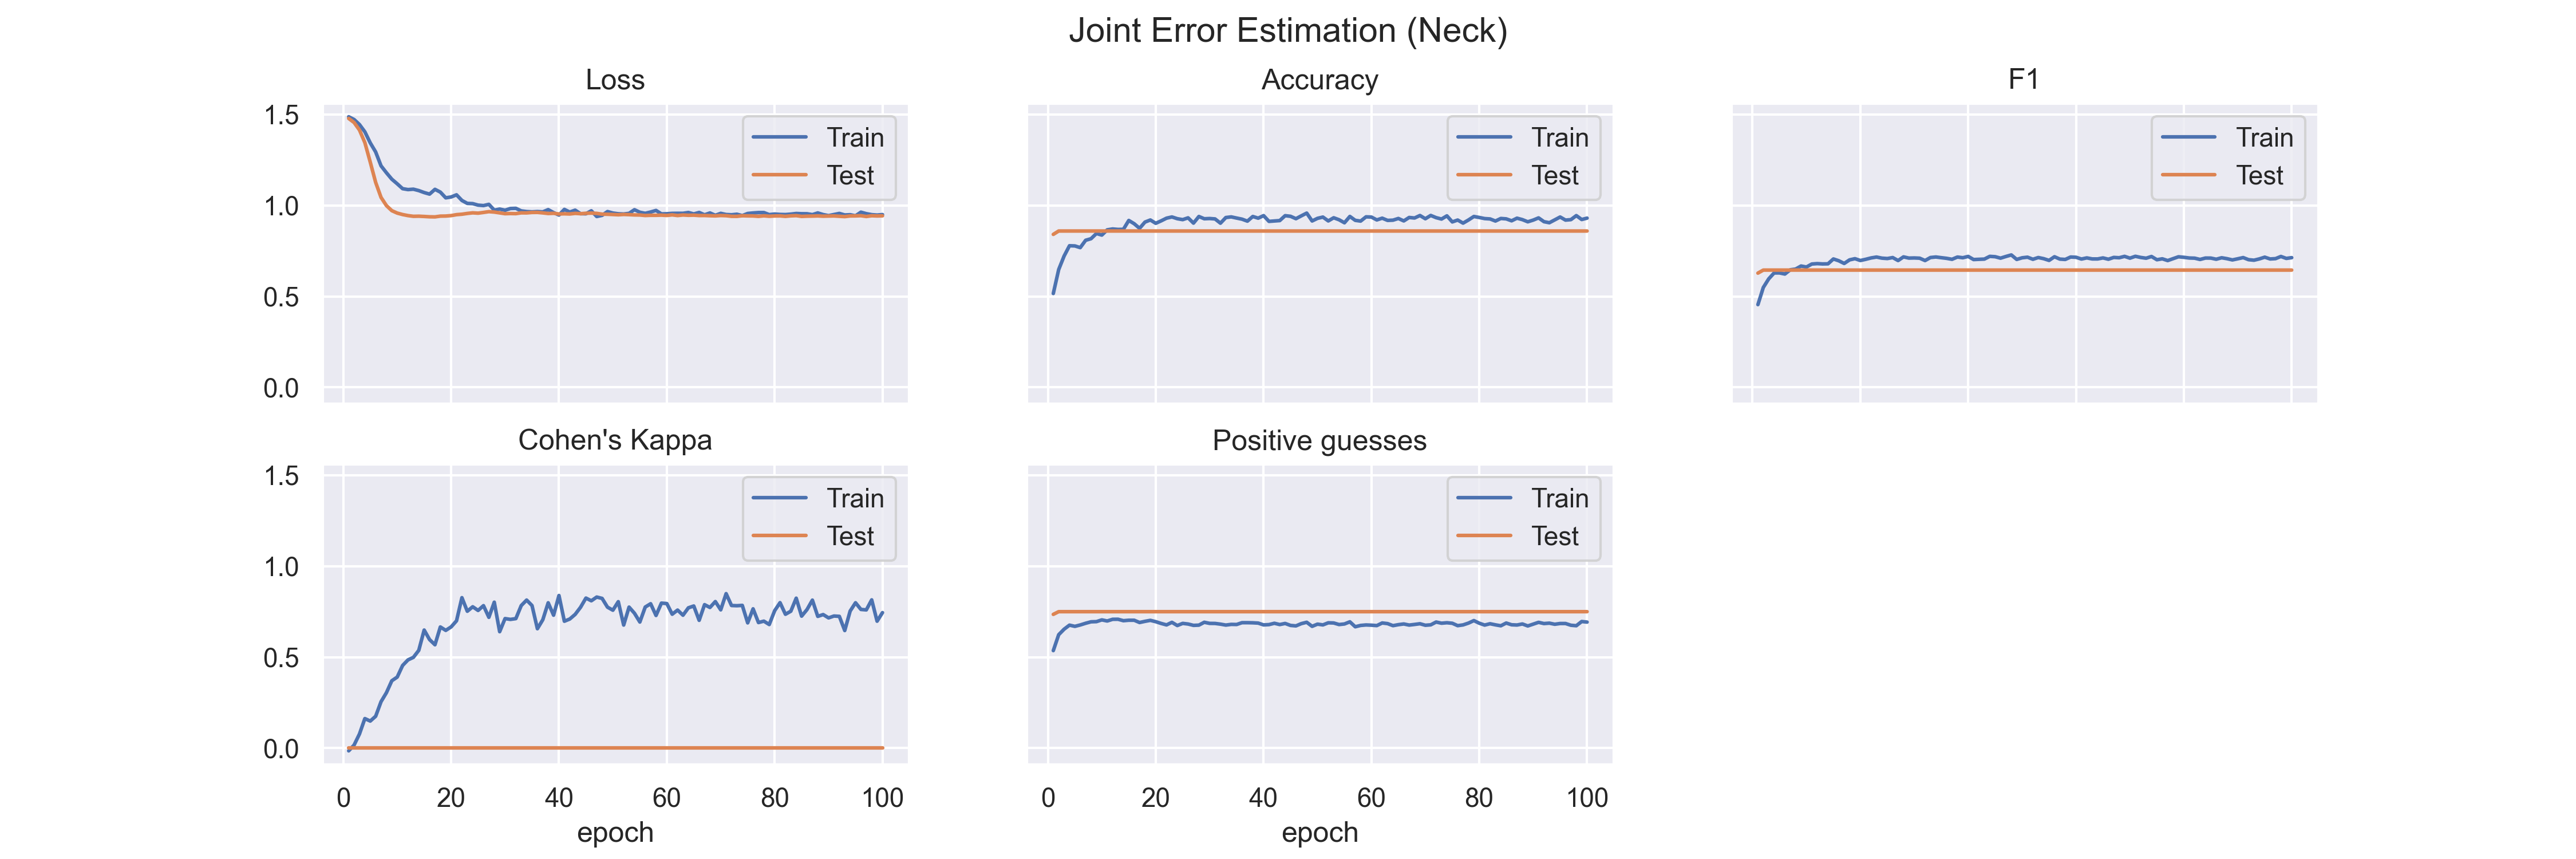
\includegraphics[width=\textwidth]{figures/Results/jt/JointErrorEstimation_Neck.png}
      \caption{Neck Error Estimation}
      \label{fig:neck_jt_ee}
  \end{subfigure}
  \hfill
  \begin{subfigure}[b]{0.47\linewidth}
      \centering
      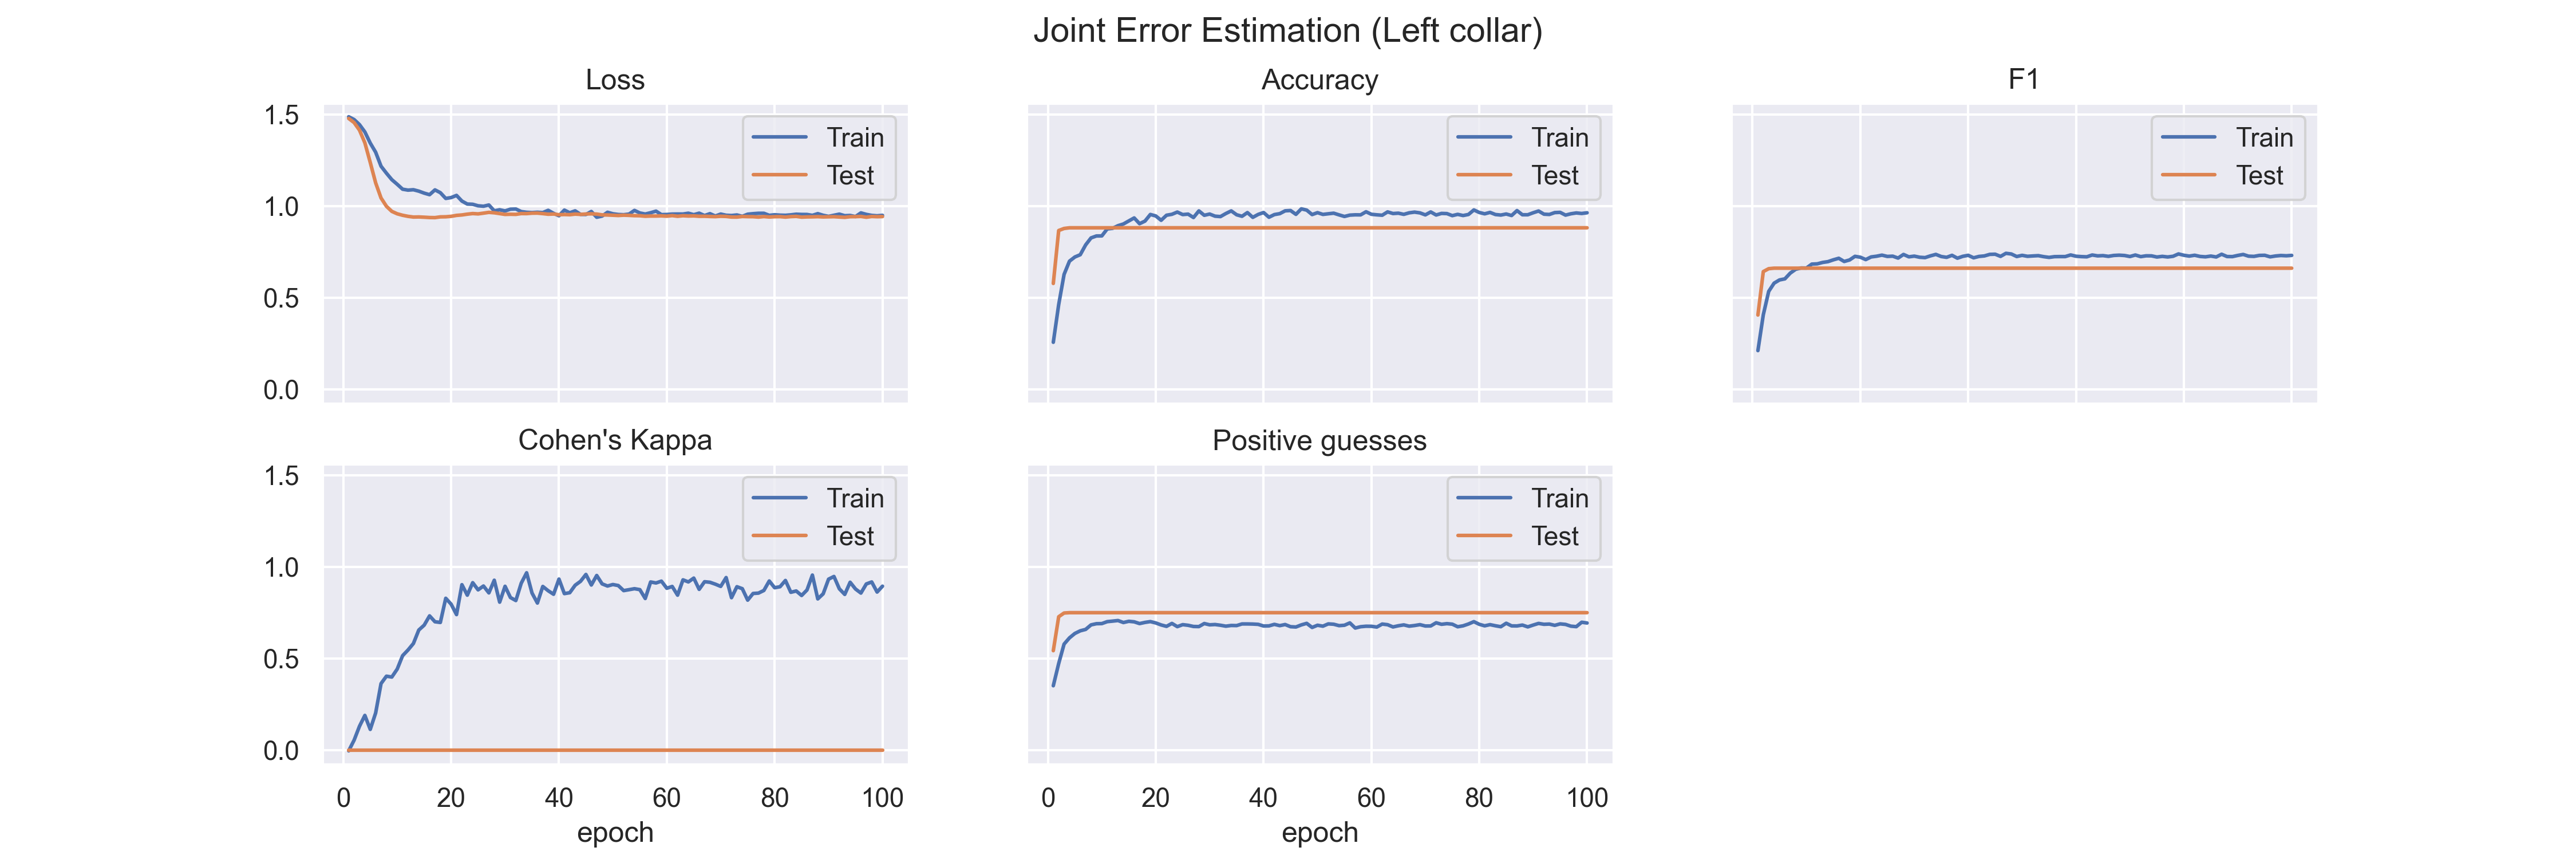
\includegraphics[width=\textwidth]{figures/Results/jt/JointErrorEstimation_Left collar.png}
      \caption{Left Collar Error Estimation}
      \label{fig:leco_jt_ee}
  \end{subfigure}
  \hfill
  \begin{subfigure}[b]{0.47\linewidth}
      \centering
      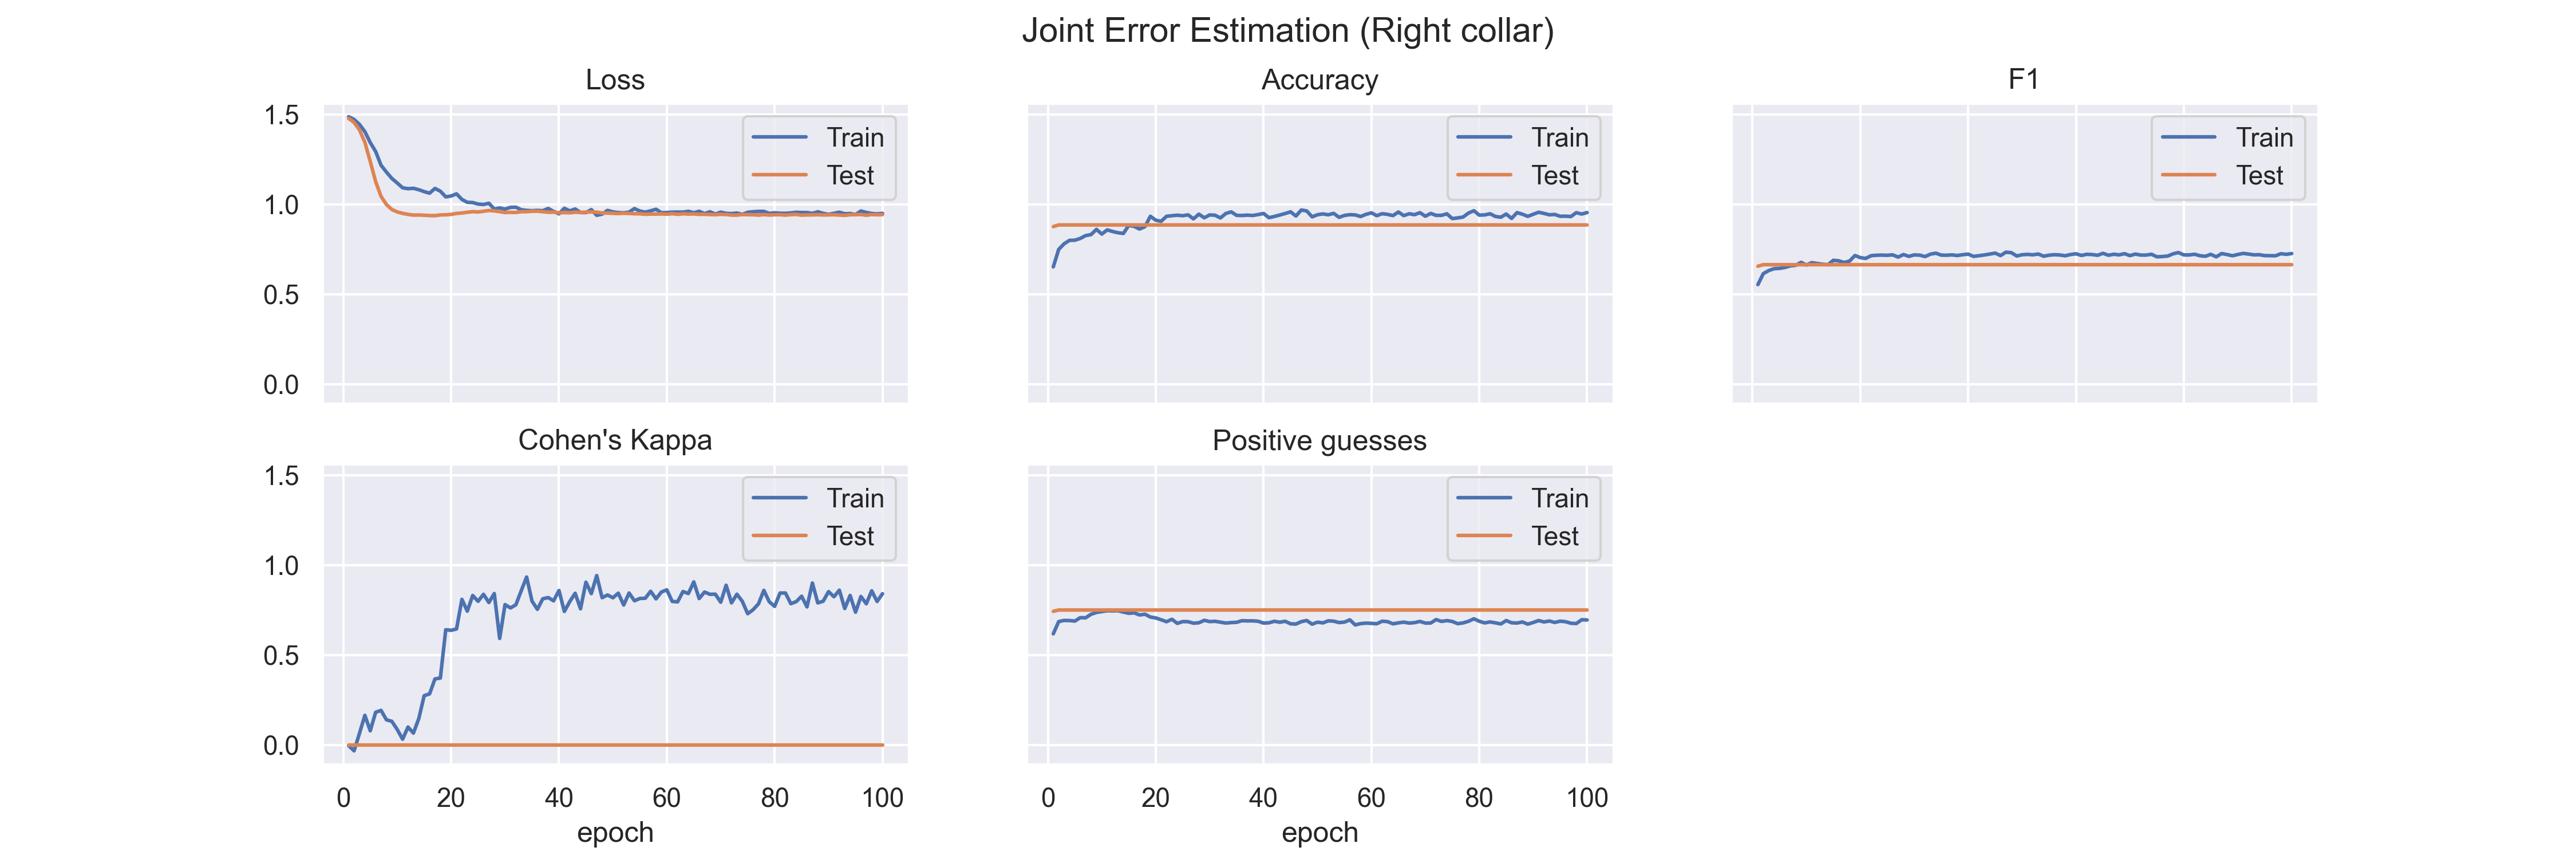
\includegraphics[width=\textwidth]{figures/Results/jt/JointErrorEstimation_Right collar.png}
      \caption{Right Collar Error Estimation}
      \label{fig:rico_jt_ee}
  \end{subfigure}
  \caption[Joint model training results]{The training results of the Joint error estimation model.}
  \label{fig:Joint_training_results}
\end{figure}


\begin{figure}
  \centering
  \begin{subfigure}[b]{0.47\linewidth}
      \centering
      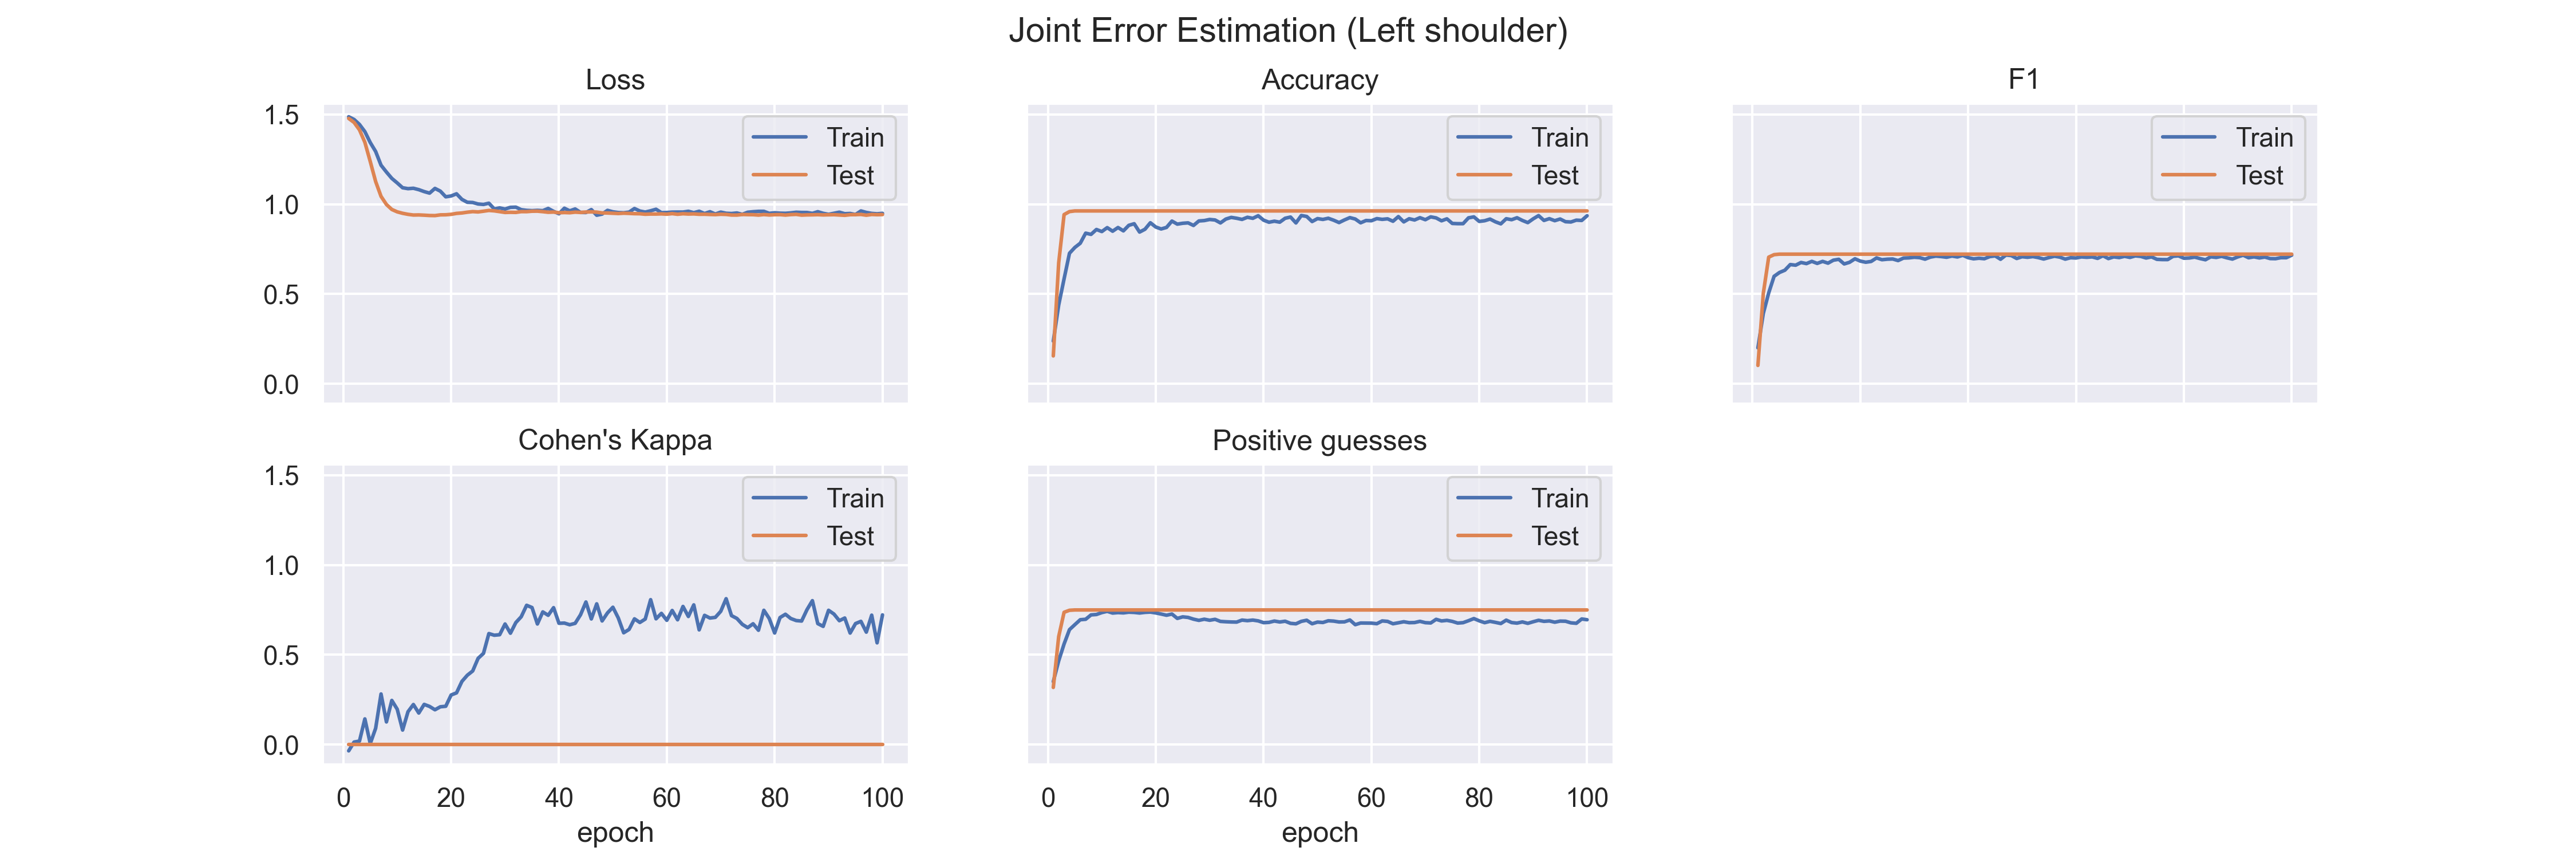
\includegraphics[width=\textwidth]{figures/Results/jt/JointErrorEstimation_Left shoulder.png}
      \caption{Left Shoulder Error Estimation}
      \label{fig:lesh_jt_ee}
  \end{subfigure}
  \hfill
  \begin{subfigure}[b]{0.47\linewidth}
      \centering
      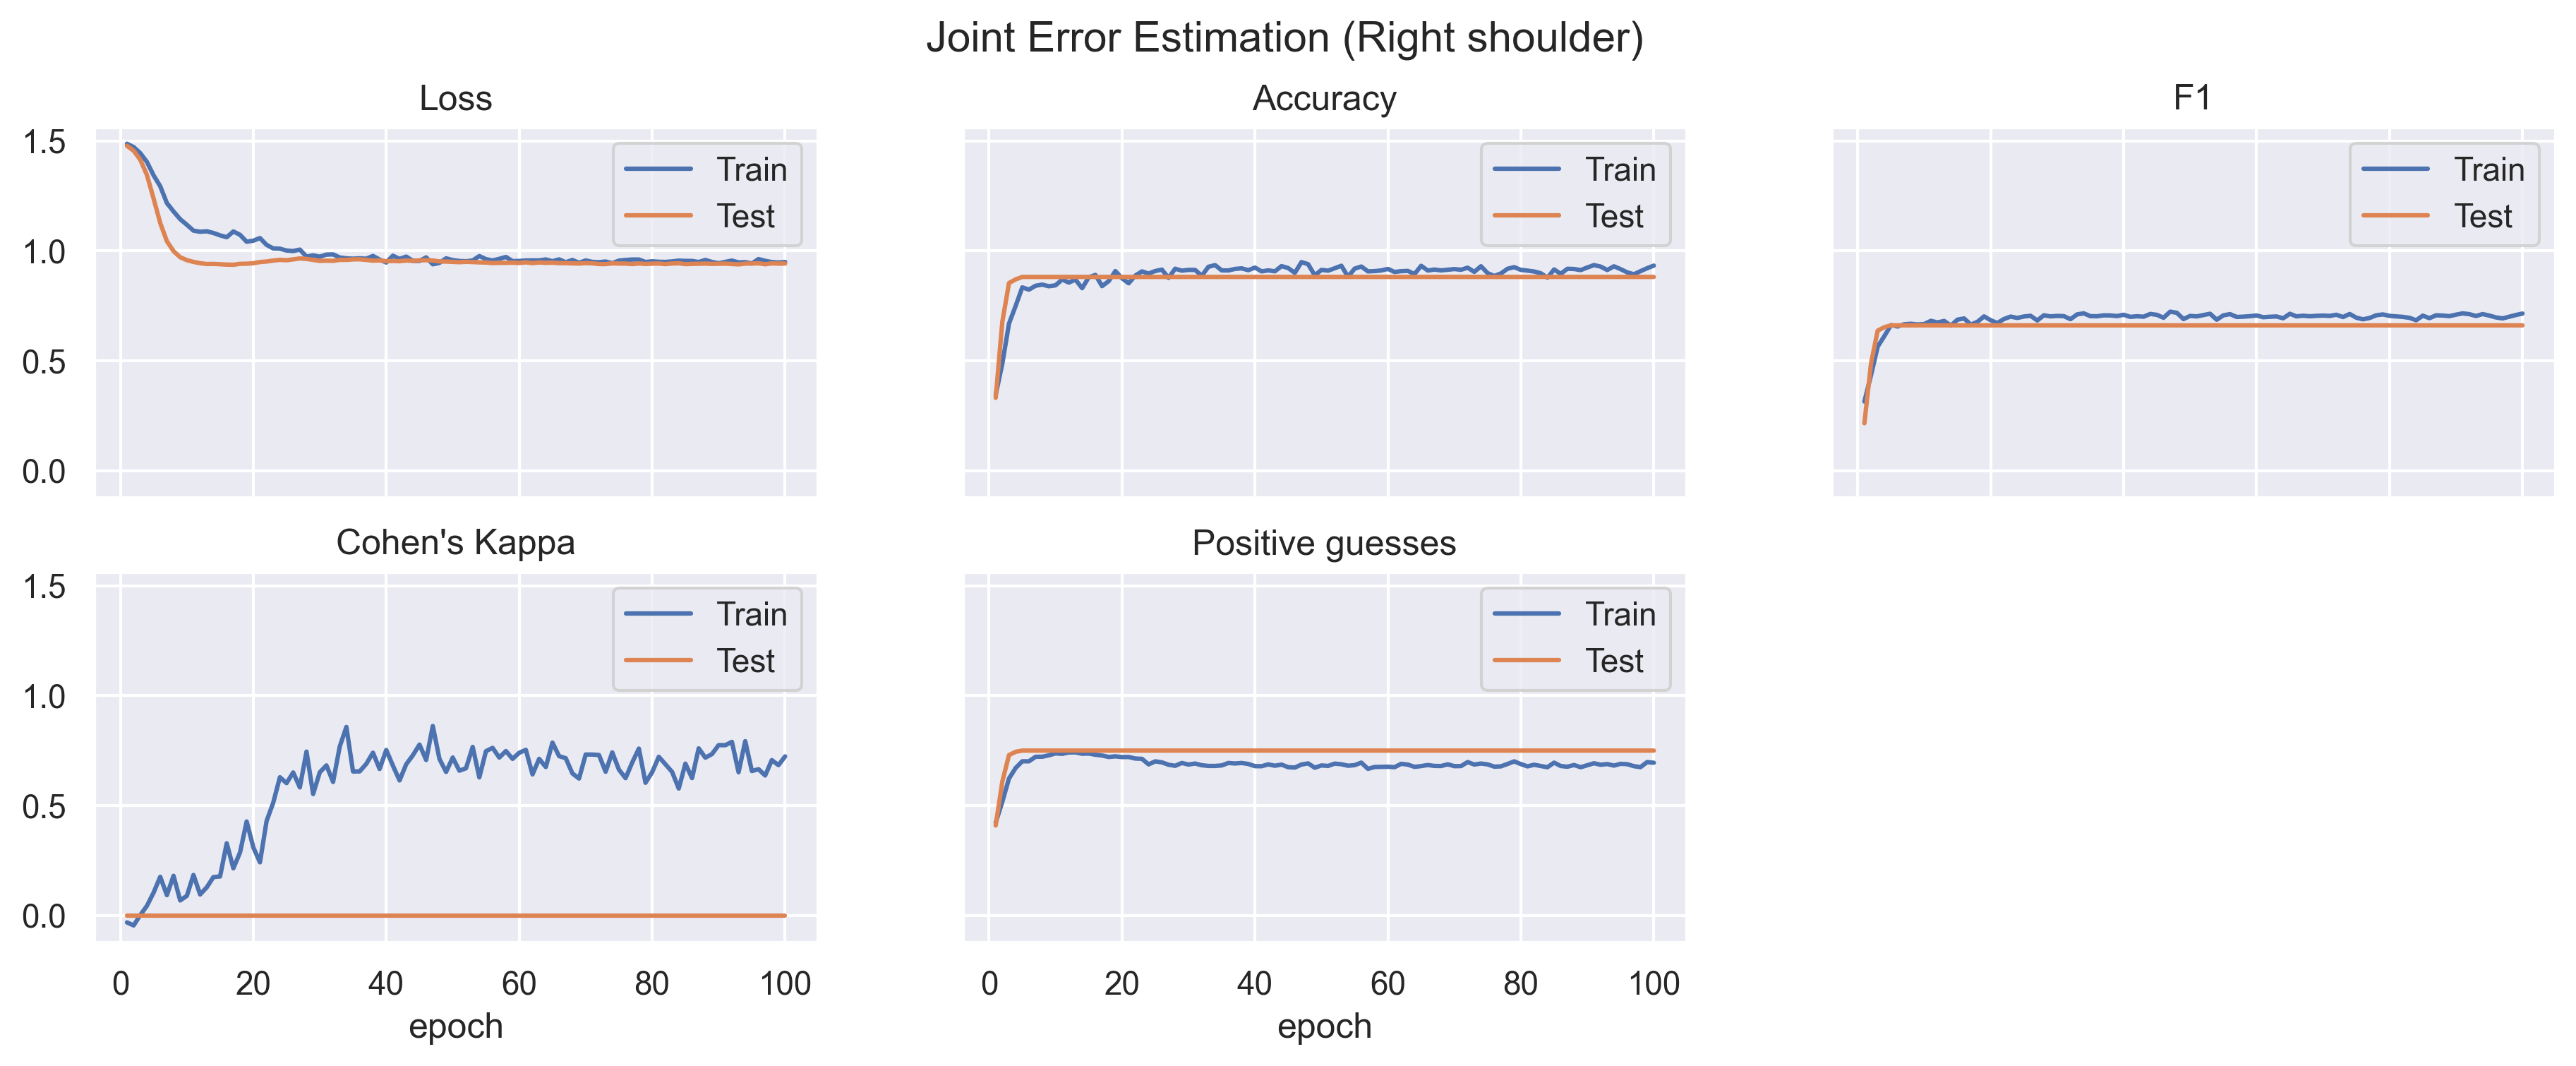
\includegraphics[width=\textwidth]{figures/Results/jt/JointErrorEstimation_Right shoulder.png}
      \caption{Right Shoulder Error Estimation}
      \label{fig:rish_jt_ee}
  \end{subfigure}
  \hfill
  \begin{subfigure}[b]{0.47\linewidth}
      \centering
      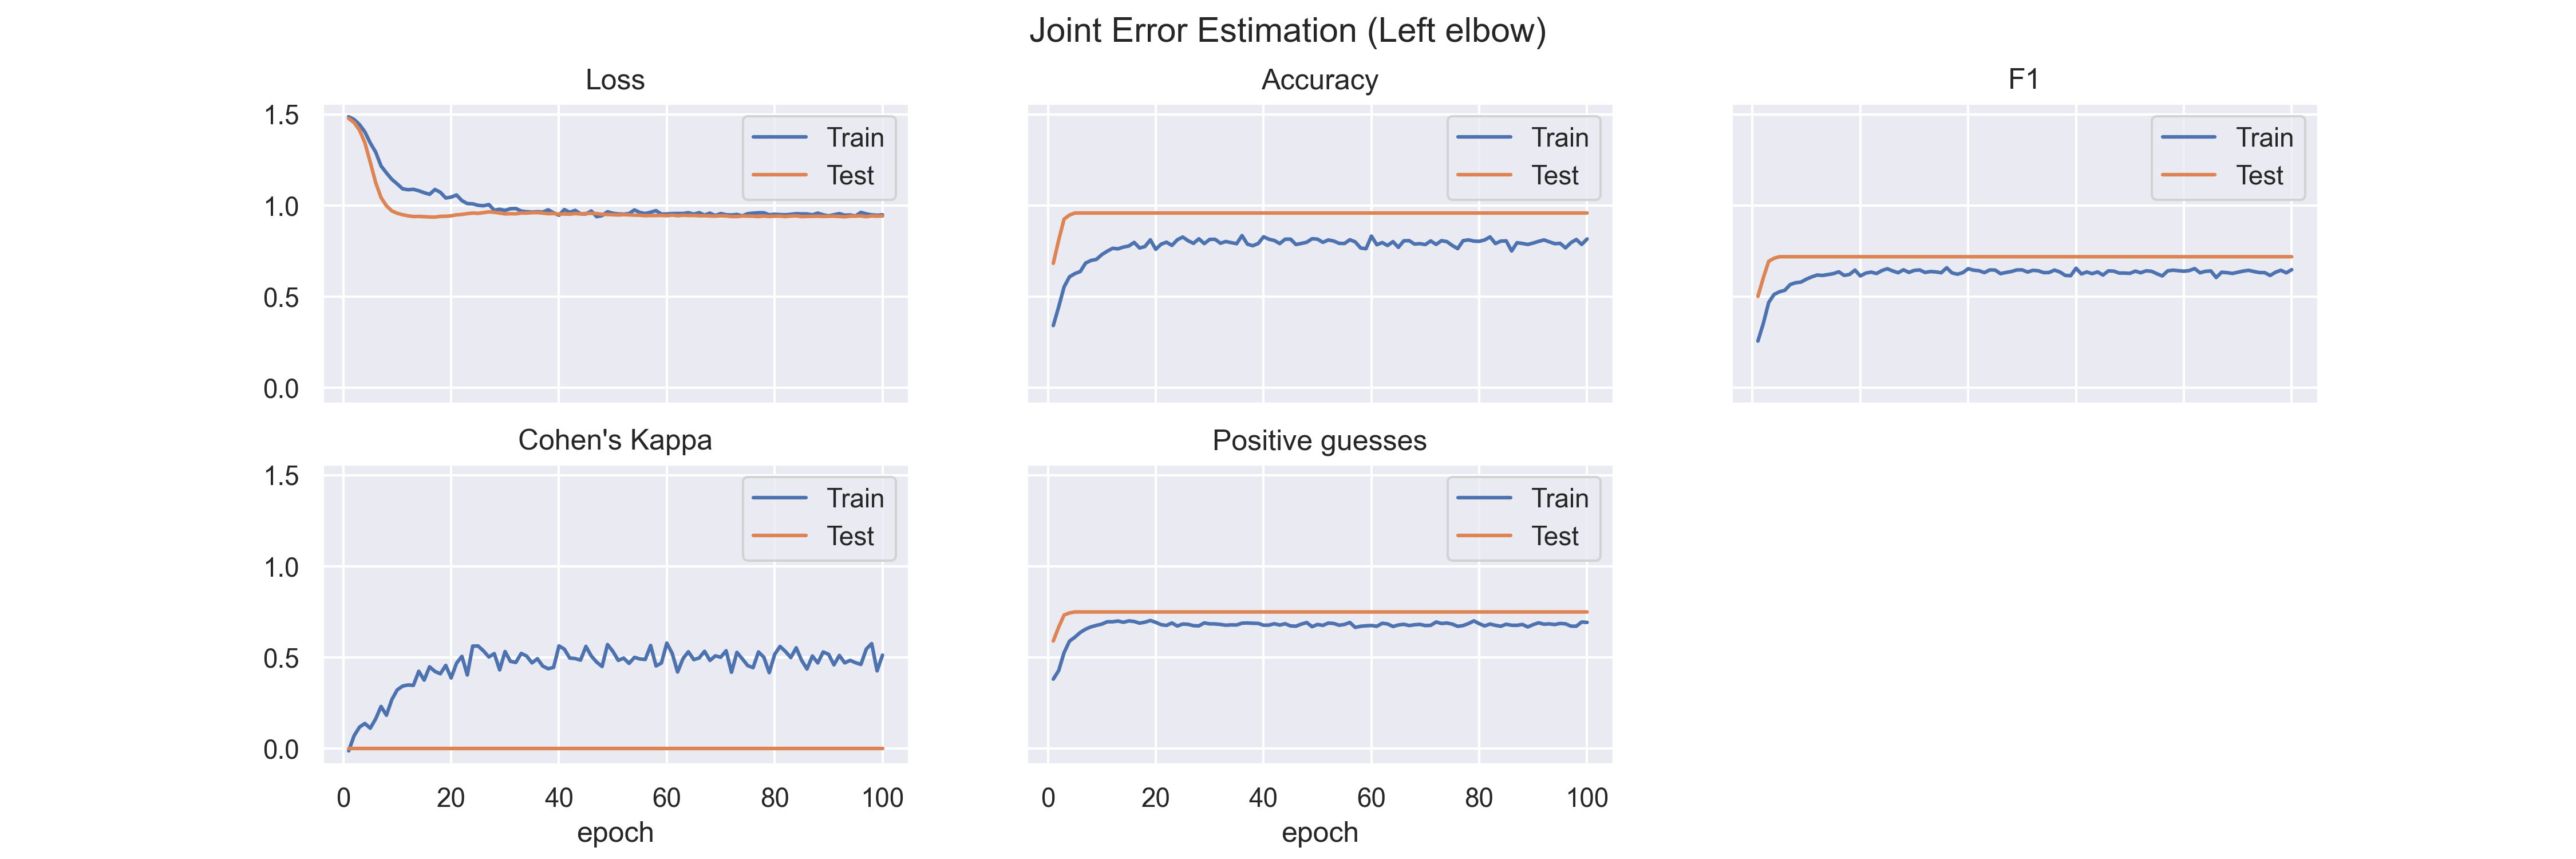
\includegraphics[width=\textwidth]{figures/Results/jt/JointErrorEstimation_Left elbow.png}
      \caption{Left Elbow Error Estimation}
      \label{fig:leel_jt_ee}
  \end{subfigure}
  \hfill
  \begin{subfigure}[b]{0.47\linewidth}
      \centering
      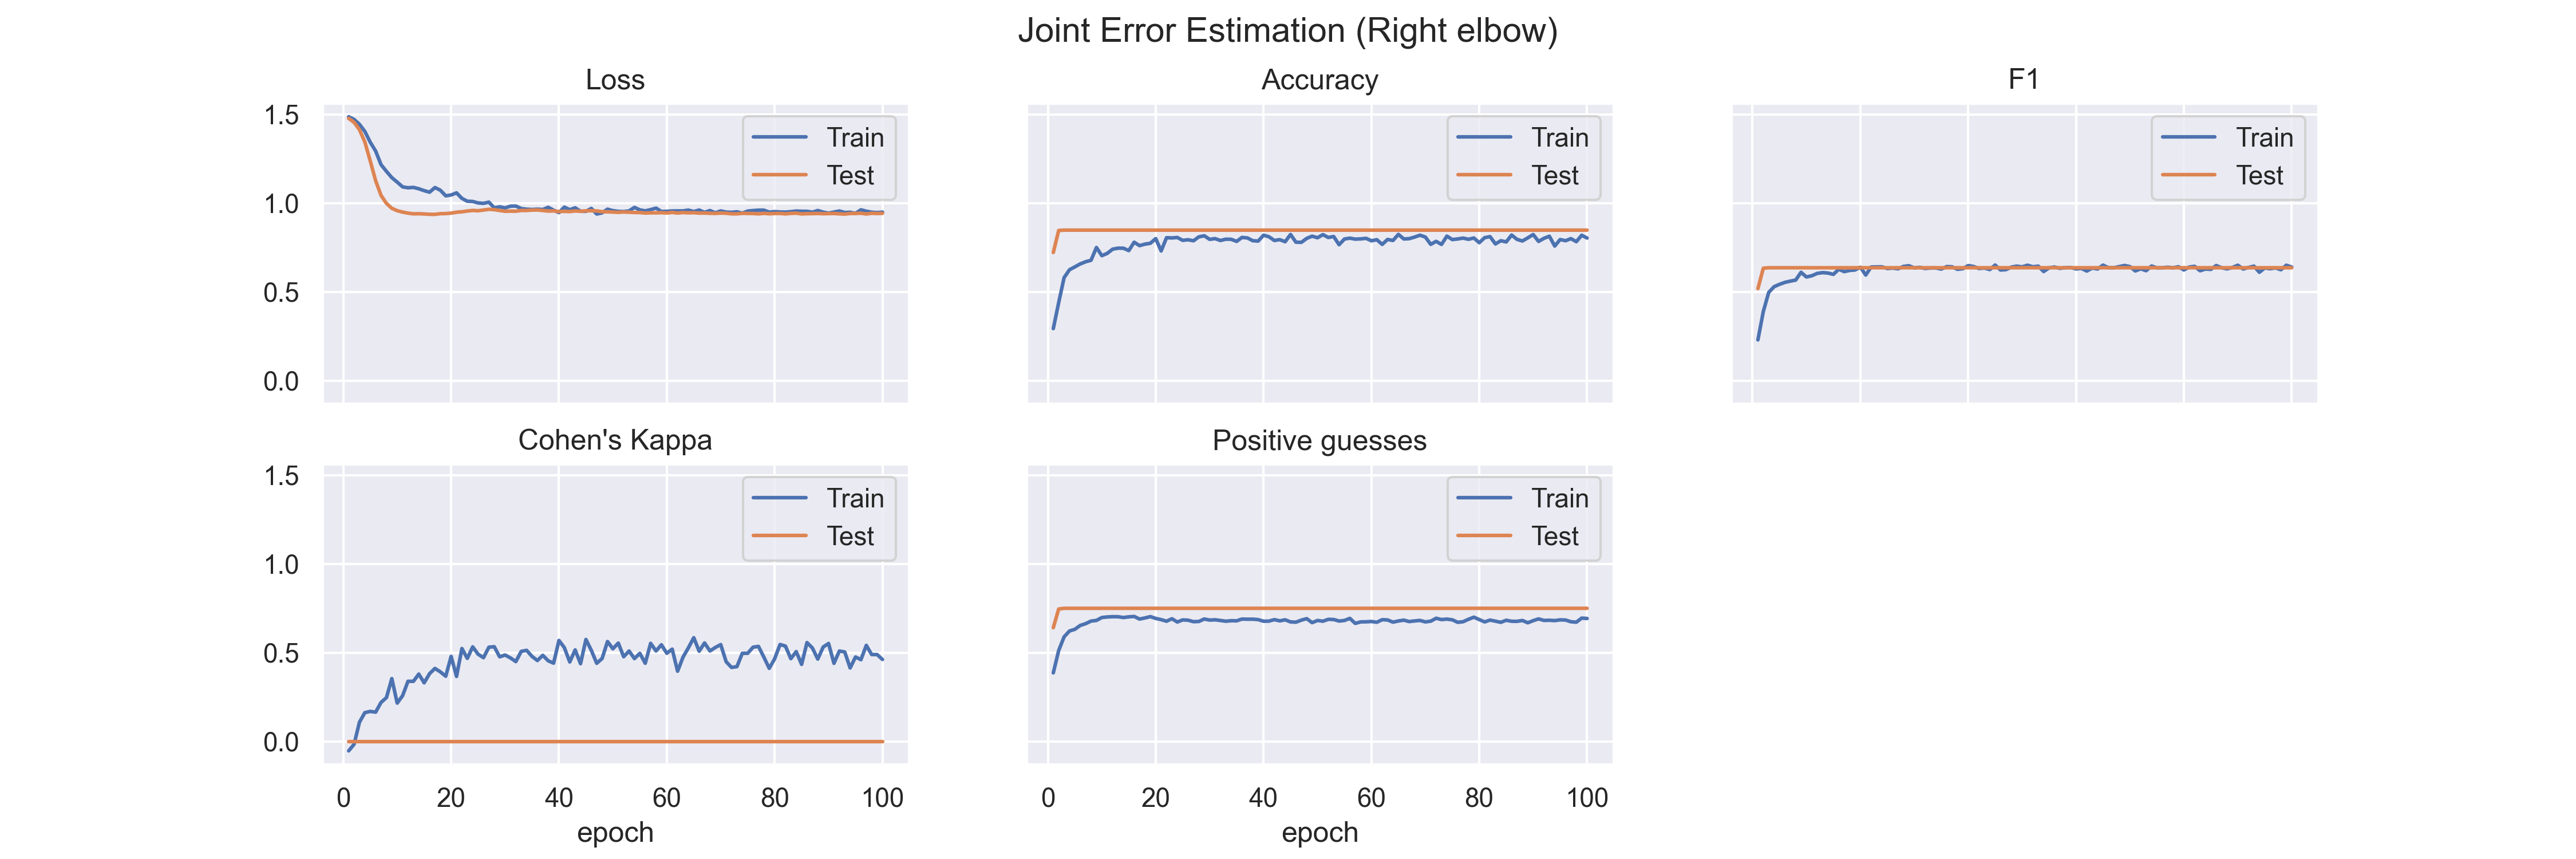
\includegraphics[width=\textwidth]{figures/Results/jt/JointErrorEstimation_Right elbow.png}
      \caption{Right Elbow Error Estimation}
      \label{fig:reel_jt_ee}
  \end{subfigure}
  \caption[Joint model training results]{The training results of the Joint error estimation model. (cont. 1)}
  \label{fig:Joint_training_results_1}
\end{figure}


\begin{figure}
  \centering
  \begin{subfigure}[b]{0.47\linewidth}
      \centering
      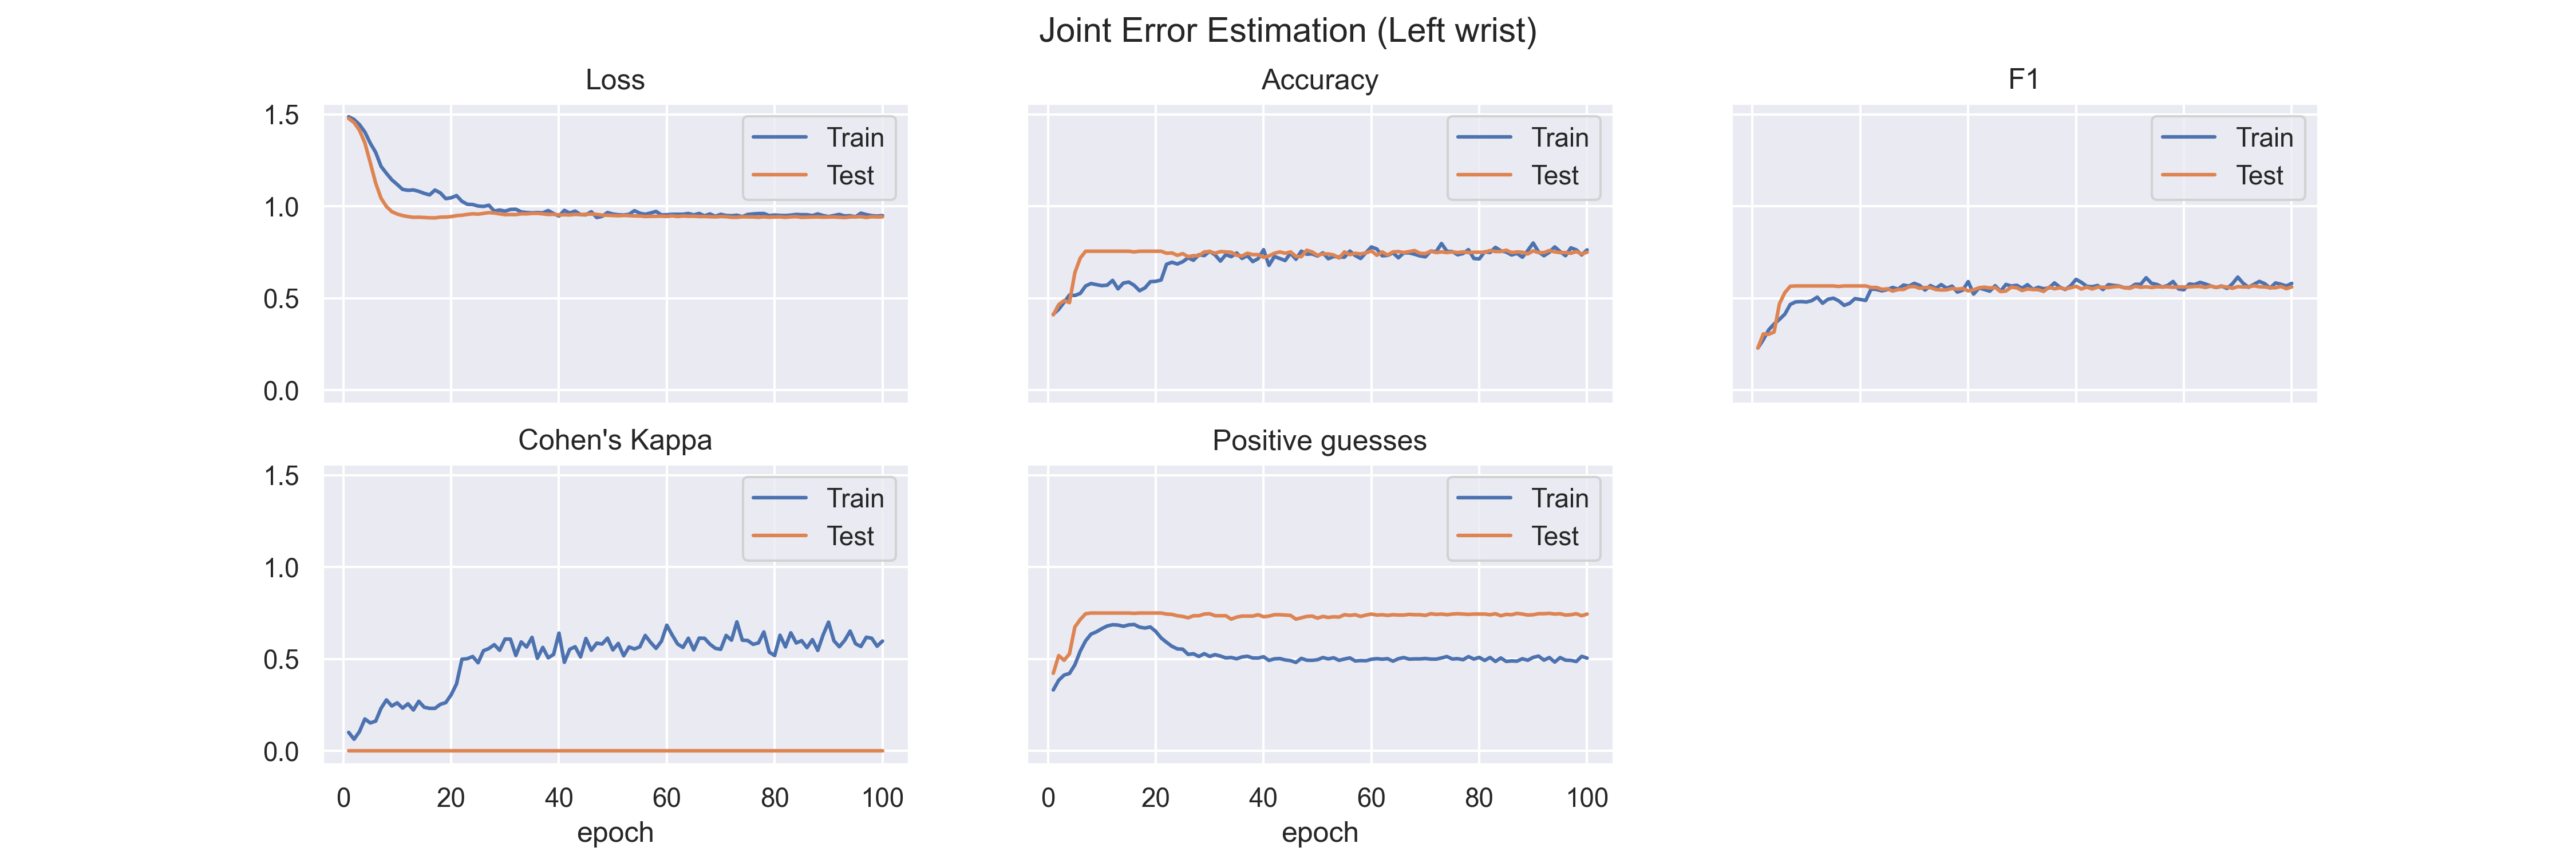
\includegraphics[width=\textwidth]{figures/Results/jt/JointErrorEstimation_Left wrist.png}
      \caption{Left Wrist Error Estimation}
      \label{fig:lewr_jt_ee}
  \end{subfigure}
  \hfill
  \begin{subfigure}[b]{0.47\linewidth}
      \centering
      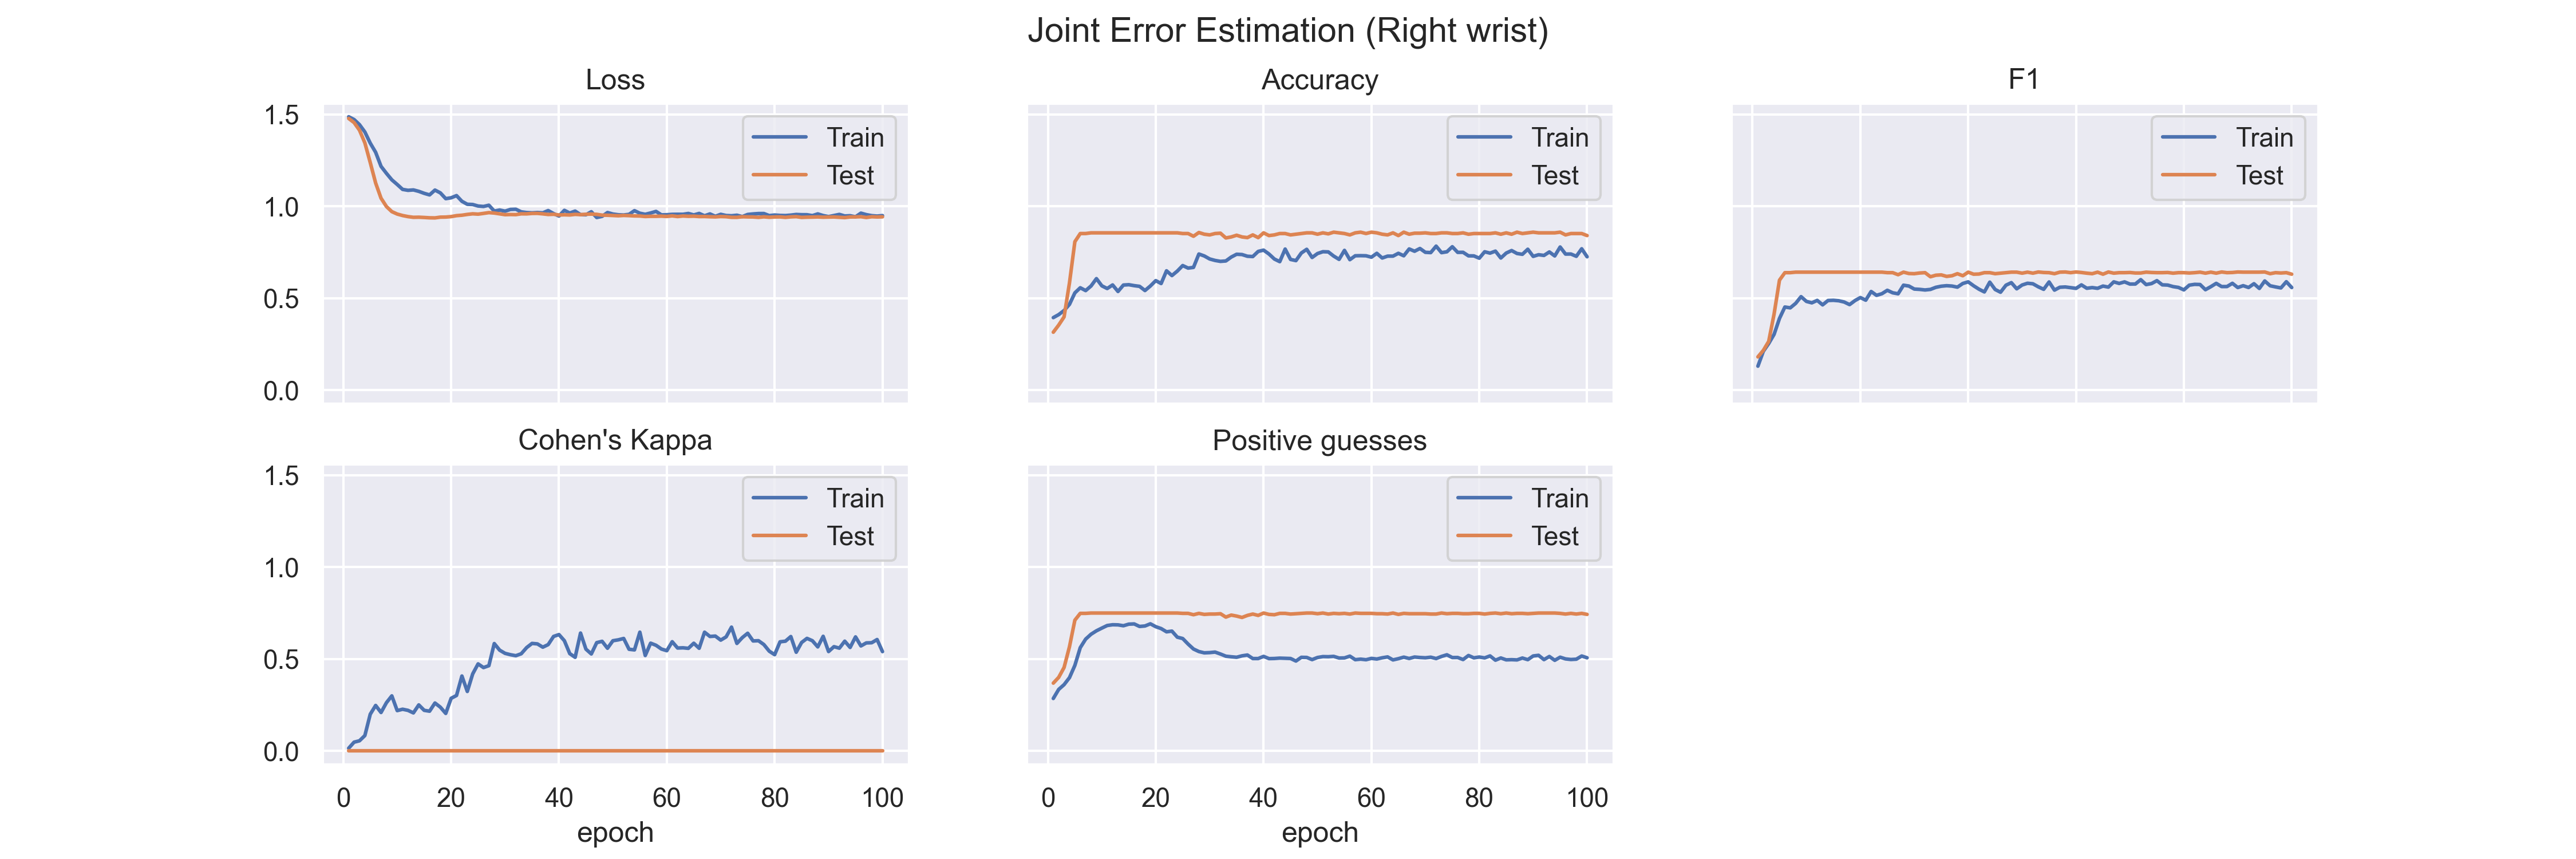
\includegraphics[width=\textwidth]{figures/Results/jt/JointErrorEstimation_Right wrist.png}
      \caption{Right Wrist Error Estimation}
      \label{fig:riwr_jt_ee}
  \end{subfigure}
  \hfill
  \begin{subfigure}[b]{0.47\linewidth}
      \centering
      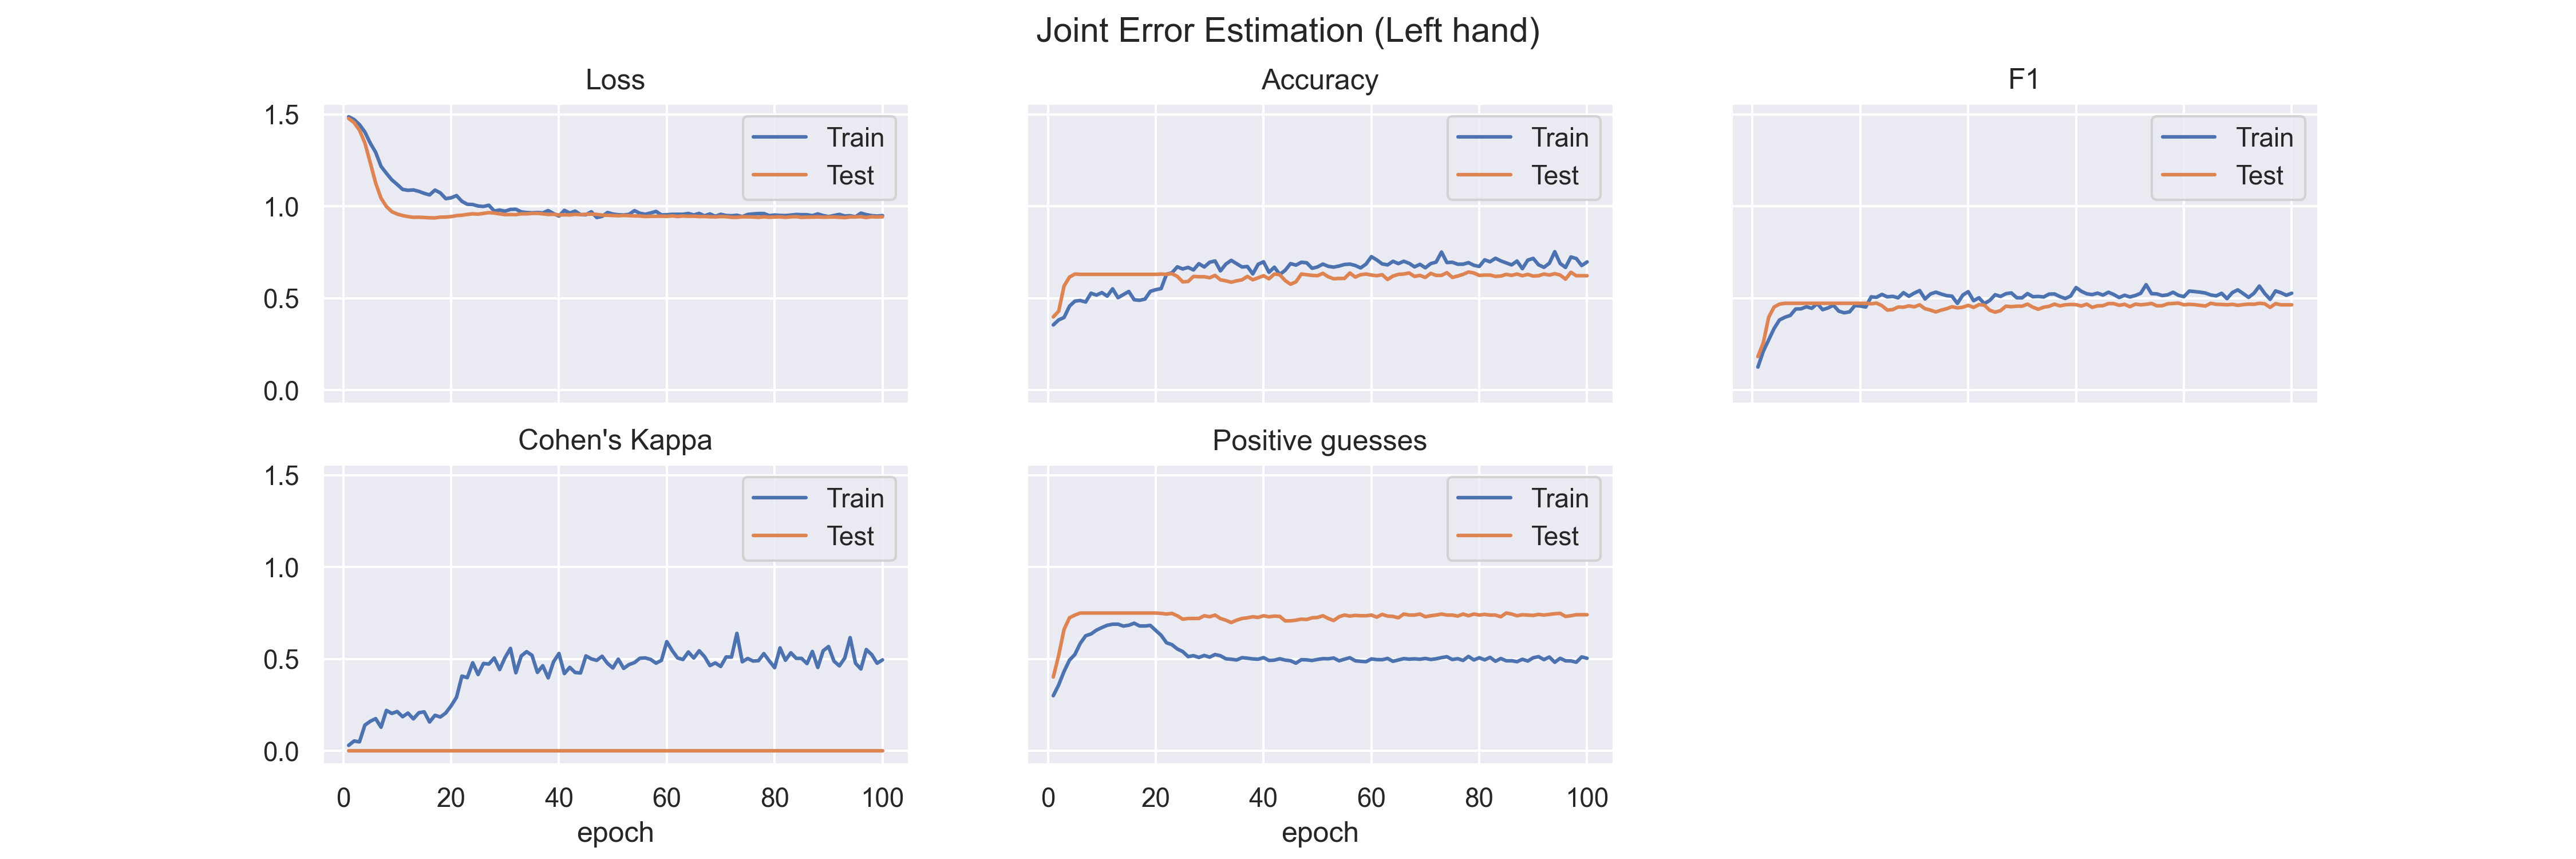
\includegraphics[width=\textwidth]{figures/Results/jt/JointErrorEstimation_Left hand.png}
      \caption{Left Hand Error Estimation}
      \label{fig:leha_jt_ee}
  \end{subfigure}
  \hfill
  \begin{subfigure}[b]{0.47\linewidth}
      \centering
      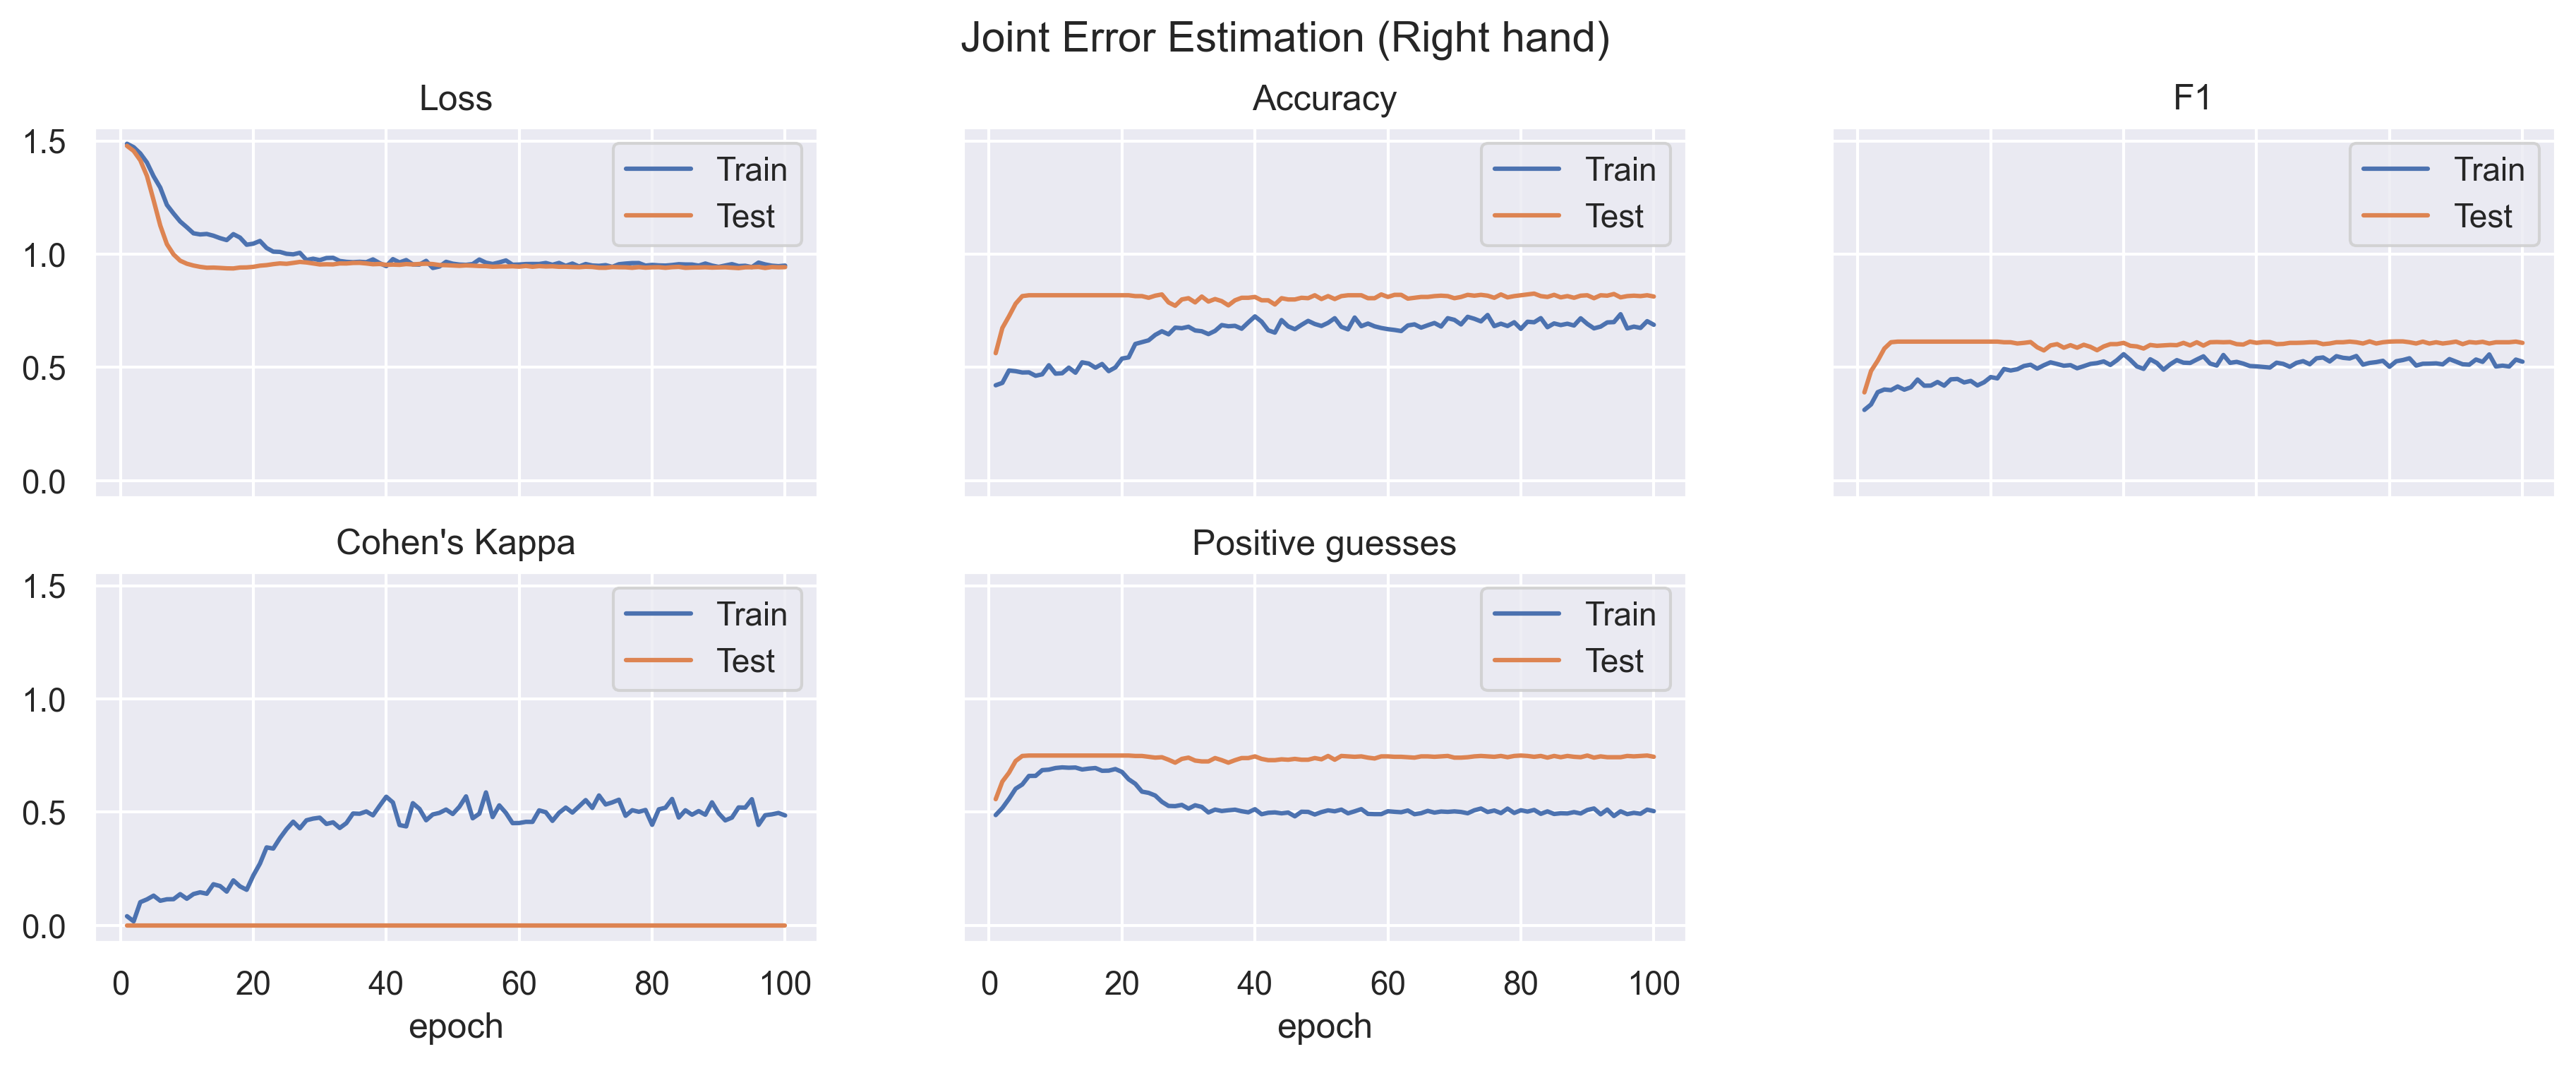
\includegraphics[width=\textwidth]{figures/Results/jt/JointErrorEstimation_Right hand.png}
      \caption{Left Arm Error Estimation}
      \label{fig:riha_jt_ee}
  \end{subfigure}
  \caption[Joint model training results]{The training results of the Joint error estimation model. (cont. 2)}
\end{figure}

\begin{figure}
  \centering
  \begin{subfigure}[b]{0.47\linewidth}
      \centering
      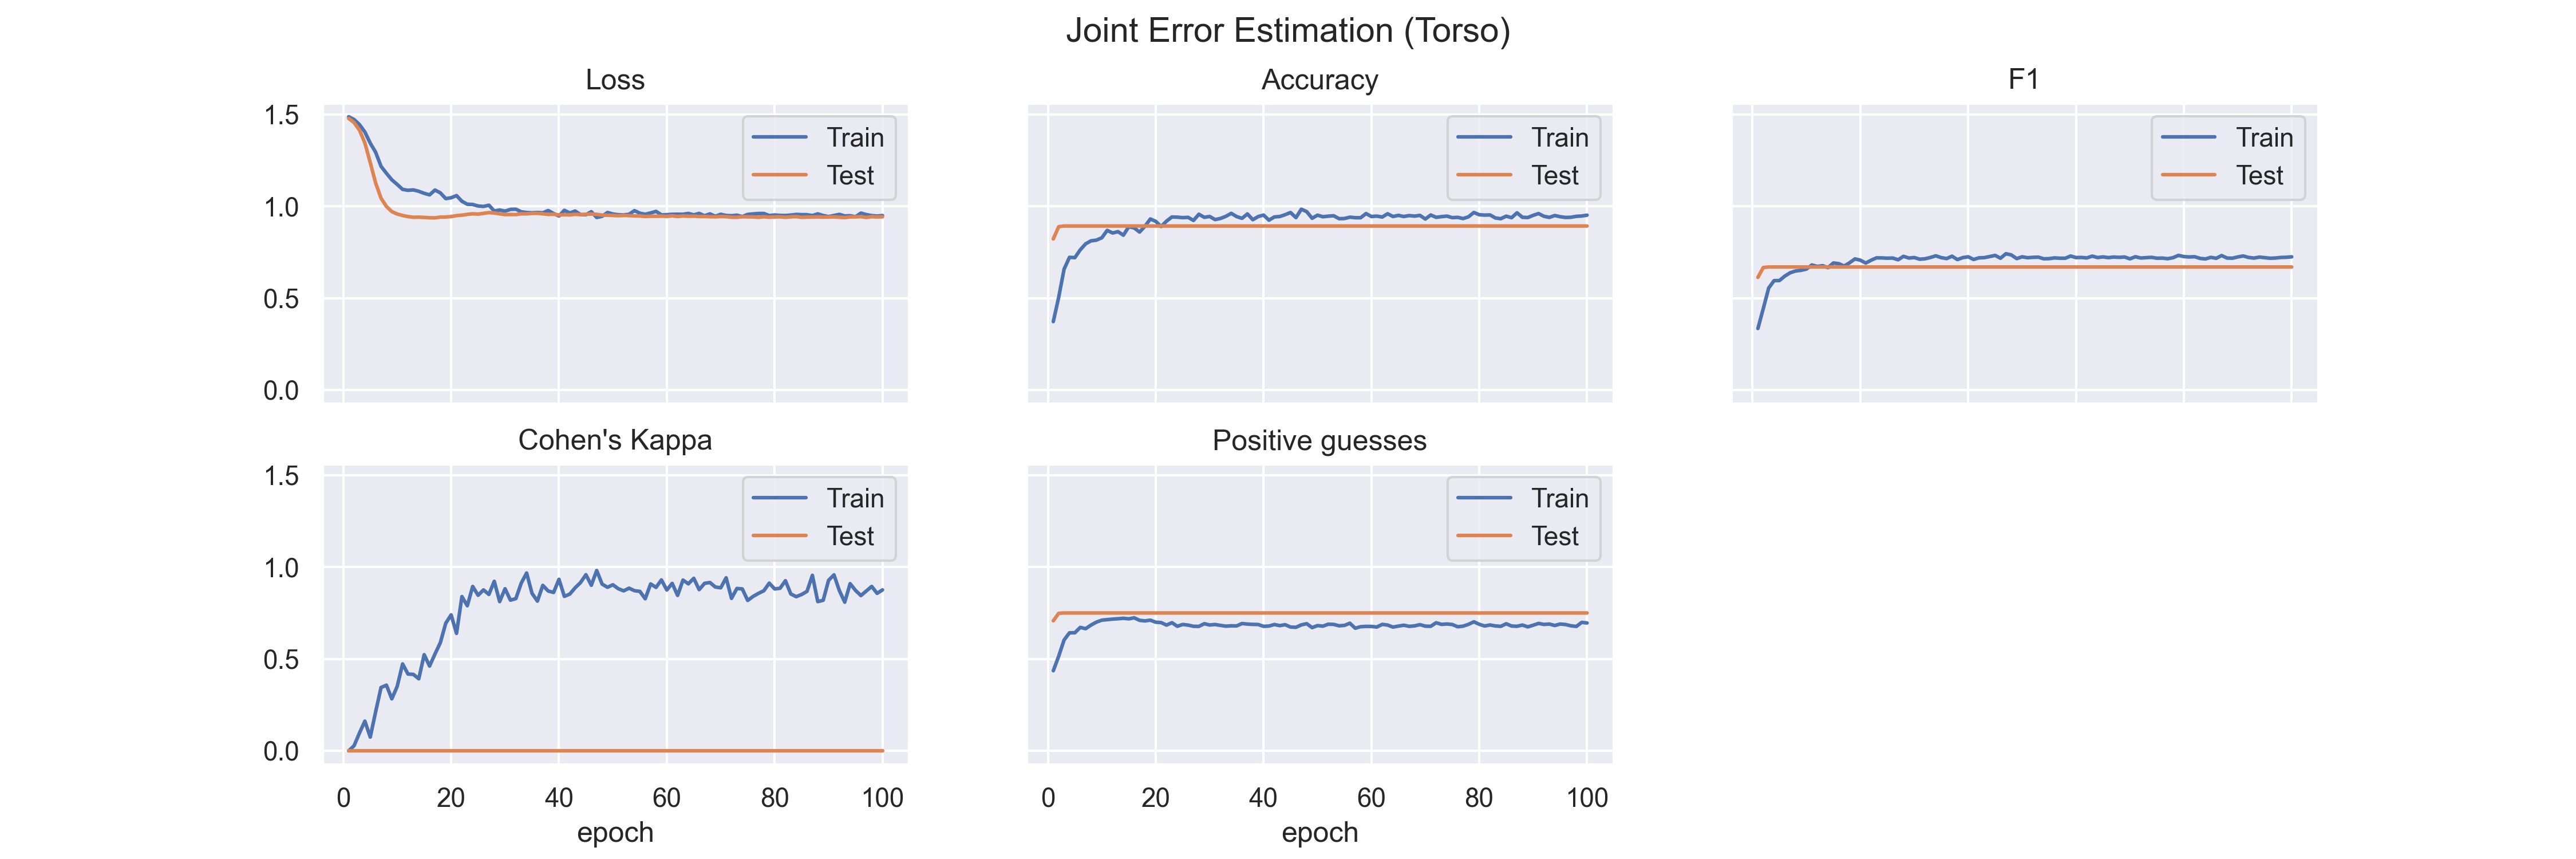
\includegraphics[width=\textwidth]{figures/Results/jt/JointErrorEstimation_Torso.png}
      \caption{Torso Error Estimation}
      \label{fig:torso_jt_ee}
  \end{subfigure}
  \hfill
  \begin{subfigure}[b]{0.47\linewidth}
    \centering
    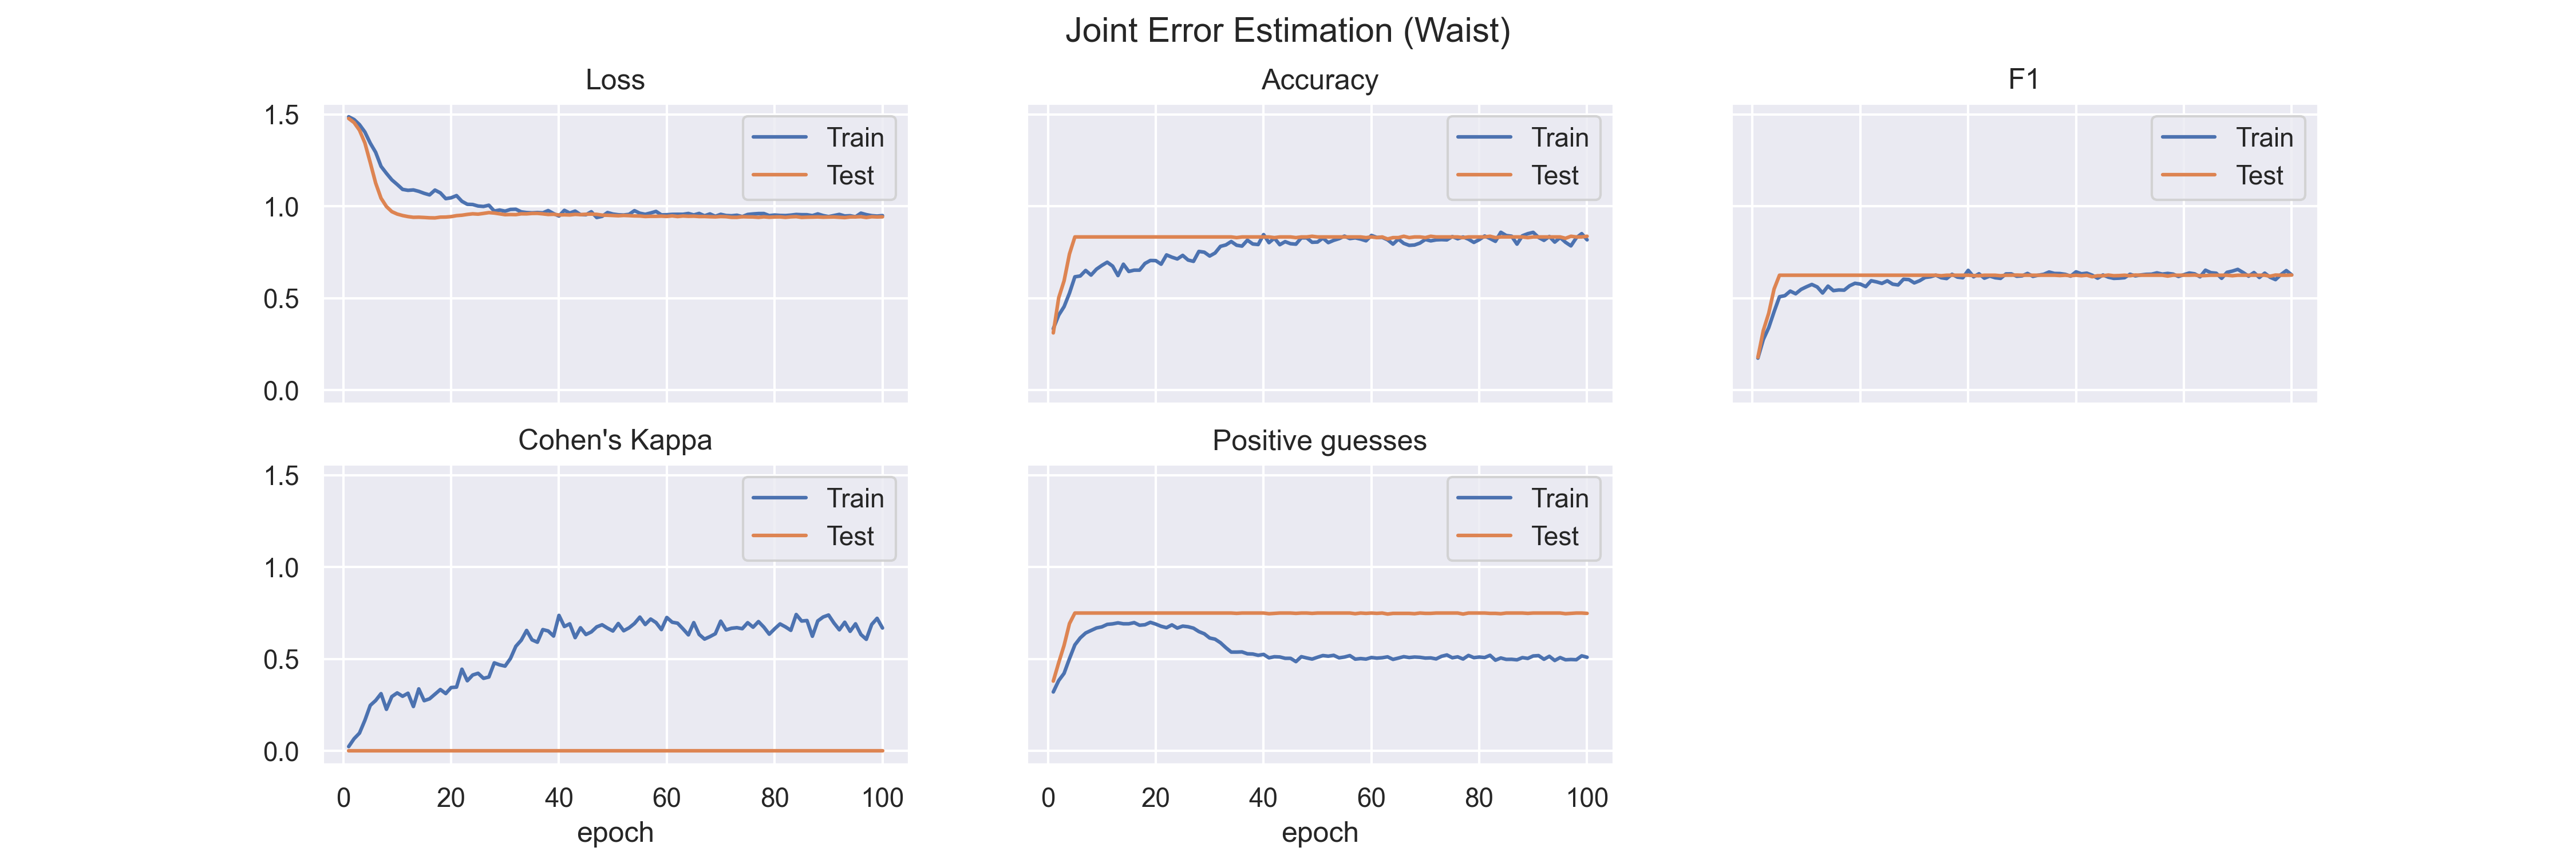
\includegraphics[width=\textwidth]{figures/Results/jt/JointErrorEstimation_Waist.png}
    \caption{Waist Error Estimation}
    \label{fig:waist_jt_ee}
  \end{subfigure}
  \hfill
  \begin{subfigure}[b]{0.47\linewidth}
      \centering
      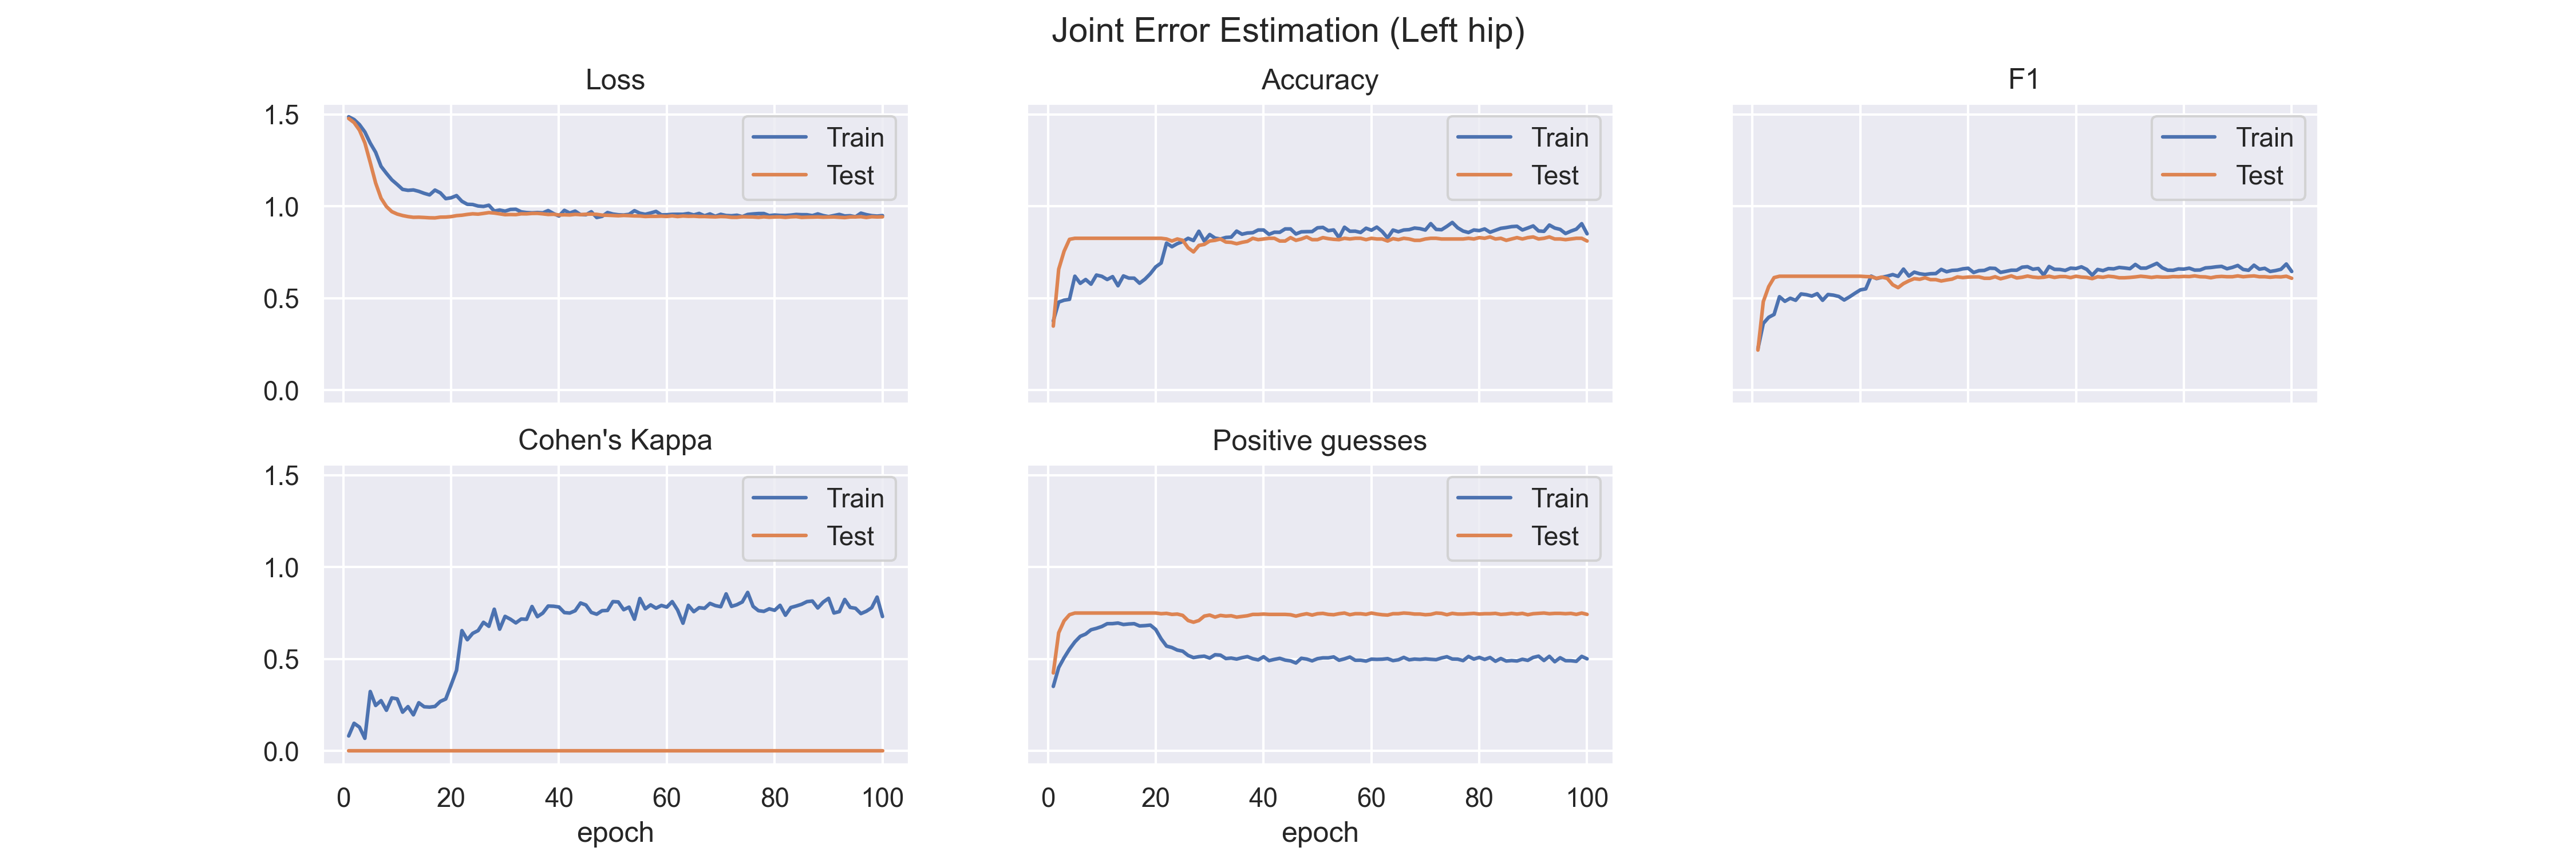
\includegraphics[width=\textwidth]{figures/Results/jt/JointErrorEstimation_Left hip.png}
      \caption{Left Hip Error Estimation}
      \label{fig:lehi_jt_ee}
  \end{subfigure}
  \hfill
  \begin{subfigure}[b]{0.47\linewidth}
      \centering
      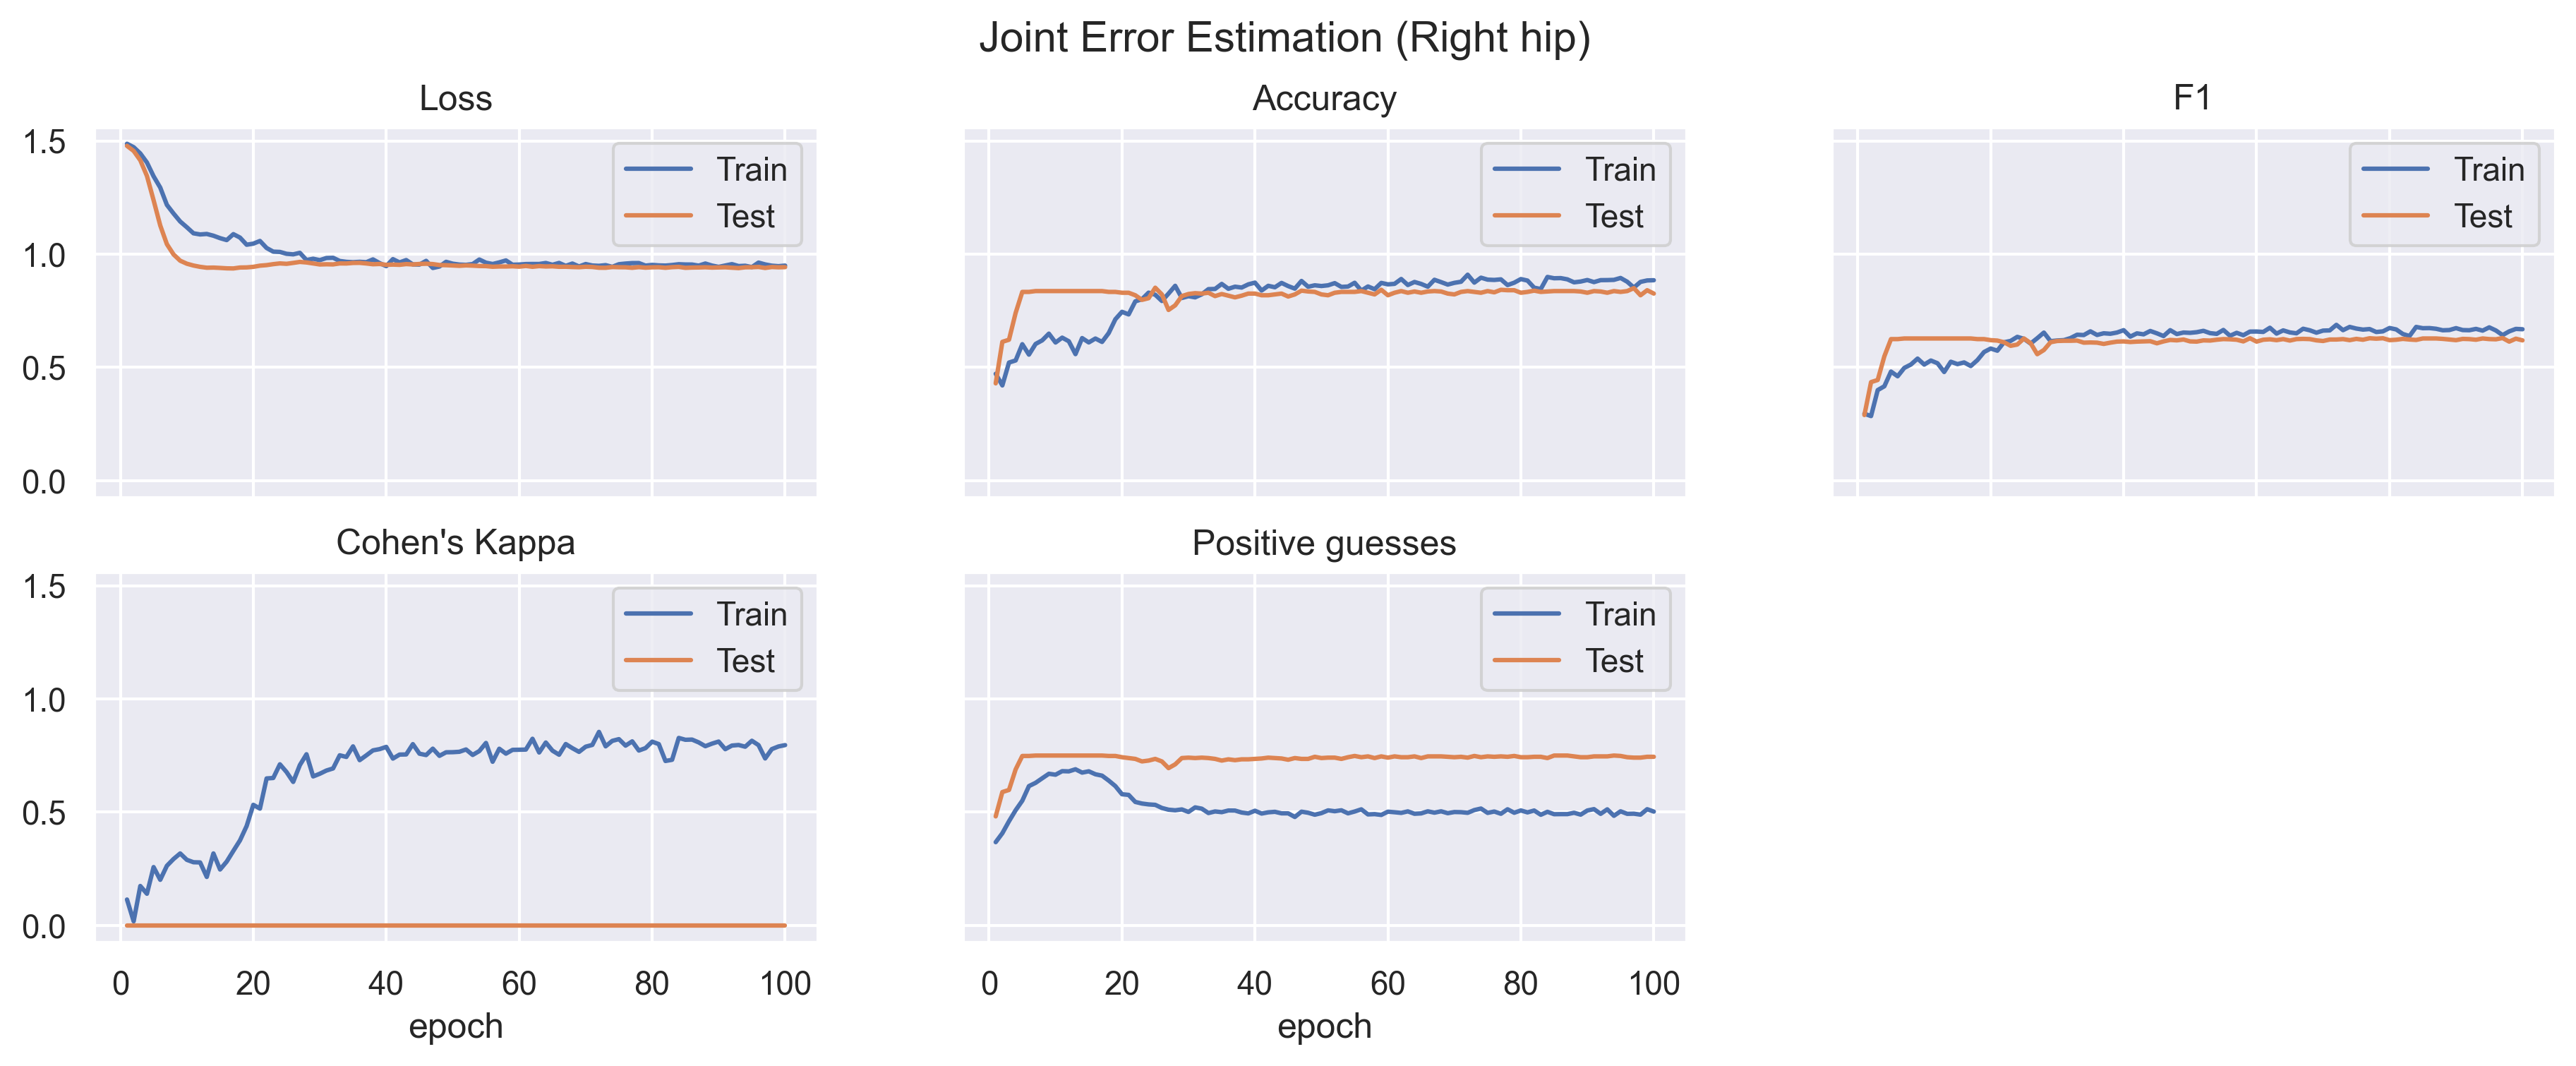
\includegraphics[width=\textwidth]{figures/Results/jt/JointErrorEstimation_Right hip.png}
      \caption{Right hip Error Estimation}
      \label{fig:rihi_jt_ee}
  \end{subfigure}
  \caption[Joint model training results]{The training results of the Joint error estimation model. (cont. 3)}
\end{figure}


\begin{figure}
  \centering
  \begin{subfigure}[b]{0.47\linewidth}
      \centering
      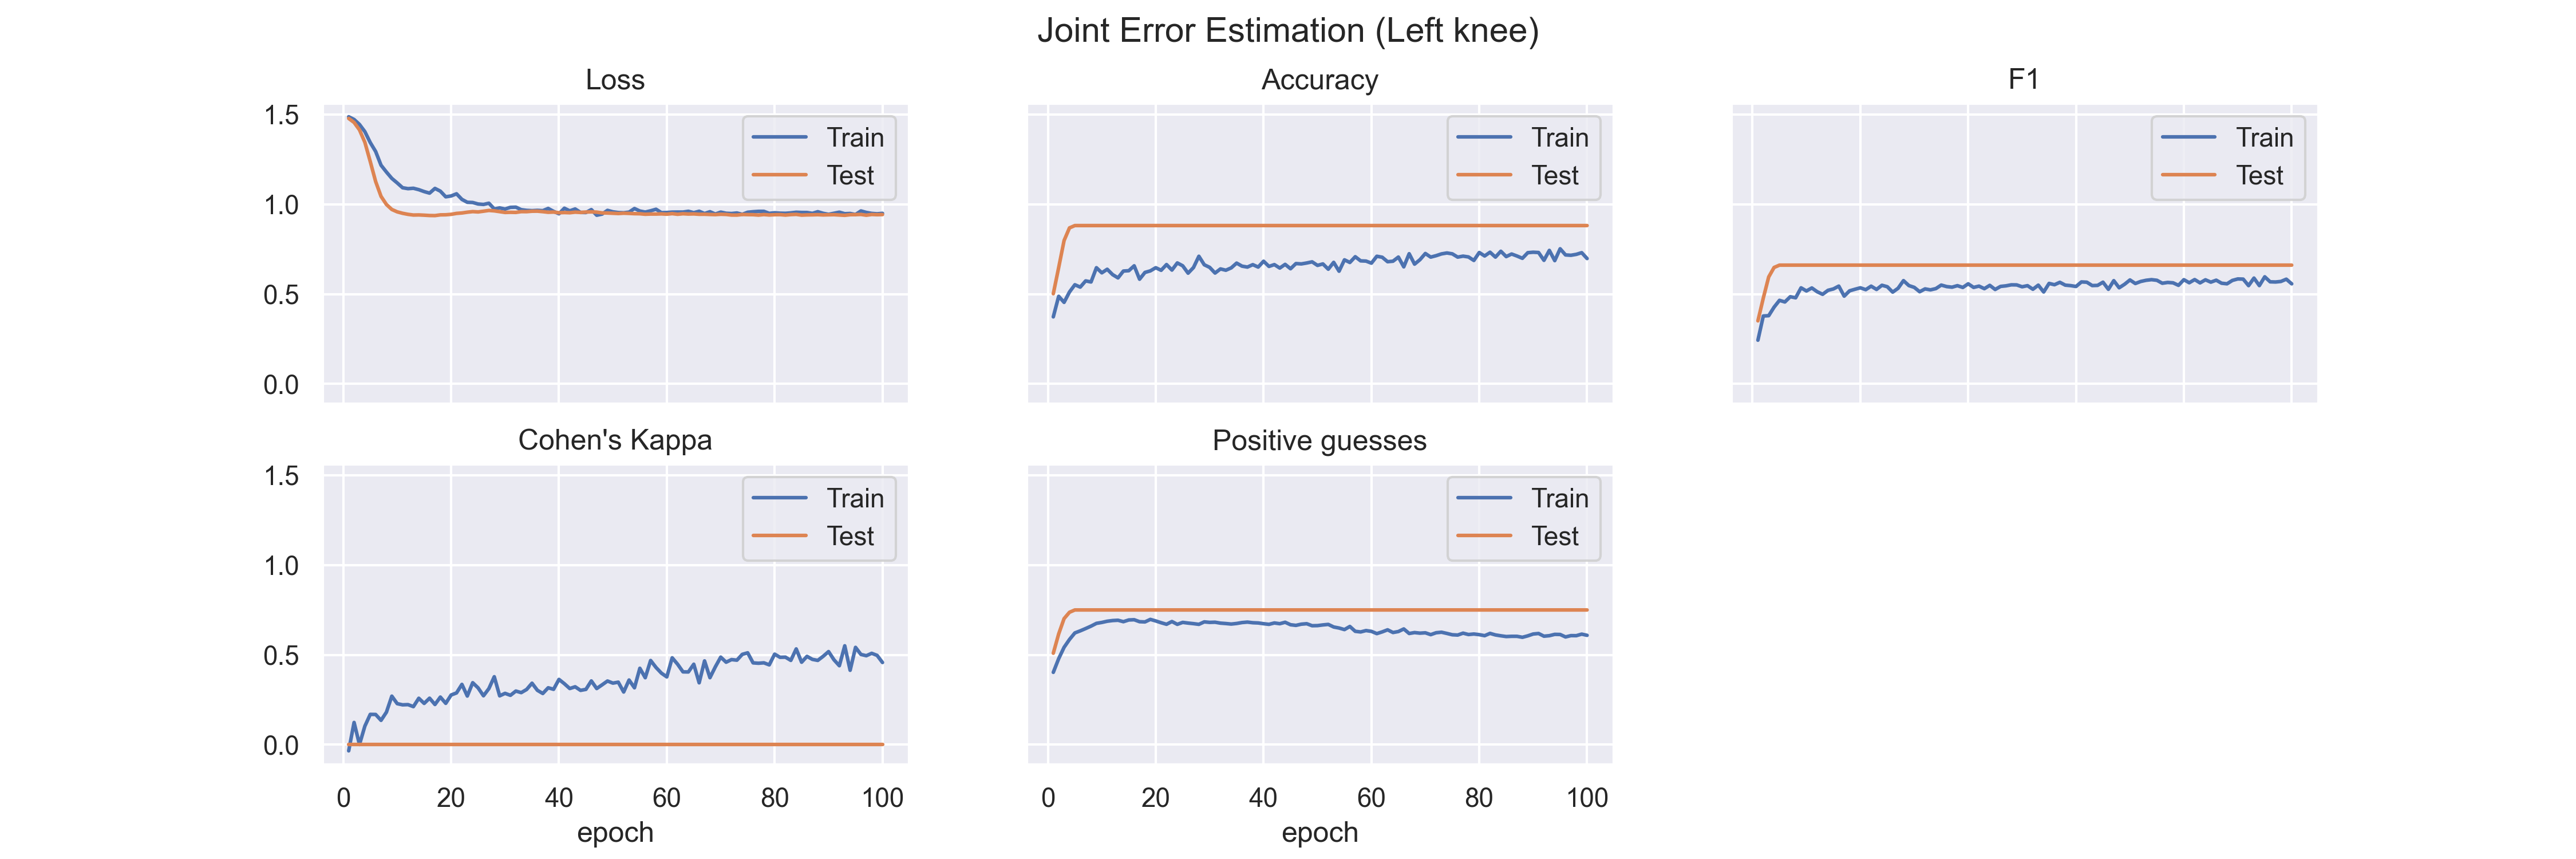
\includegraphics[width=\textwidth]{figures/Results/jt/JointErrorEstimation_Left knee.png}
      \caption{left Knee Error Estimation}
      \label{fig:lekn_jt_ee}
  \end{subfigure}
  \hfill
  \begin{subfigure}[b]{0.47\linewidth}
      \centering
      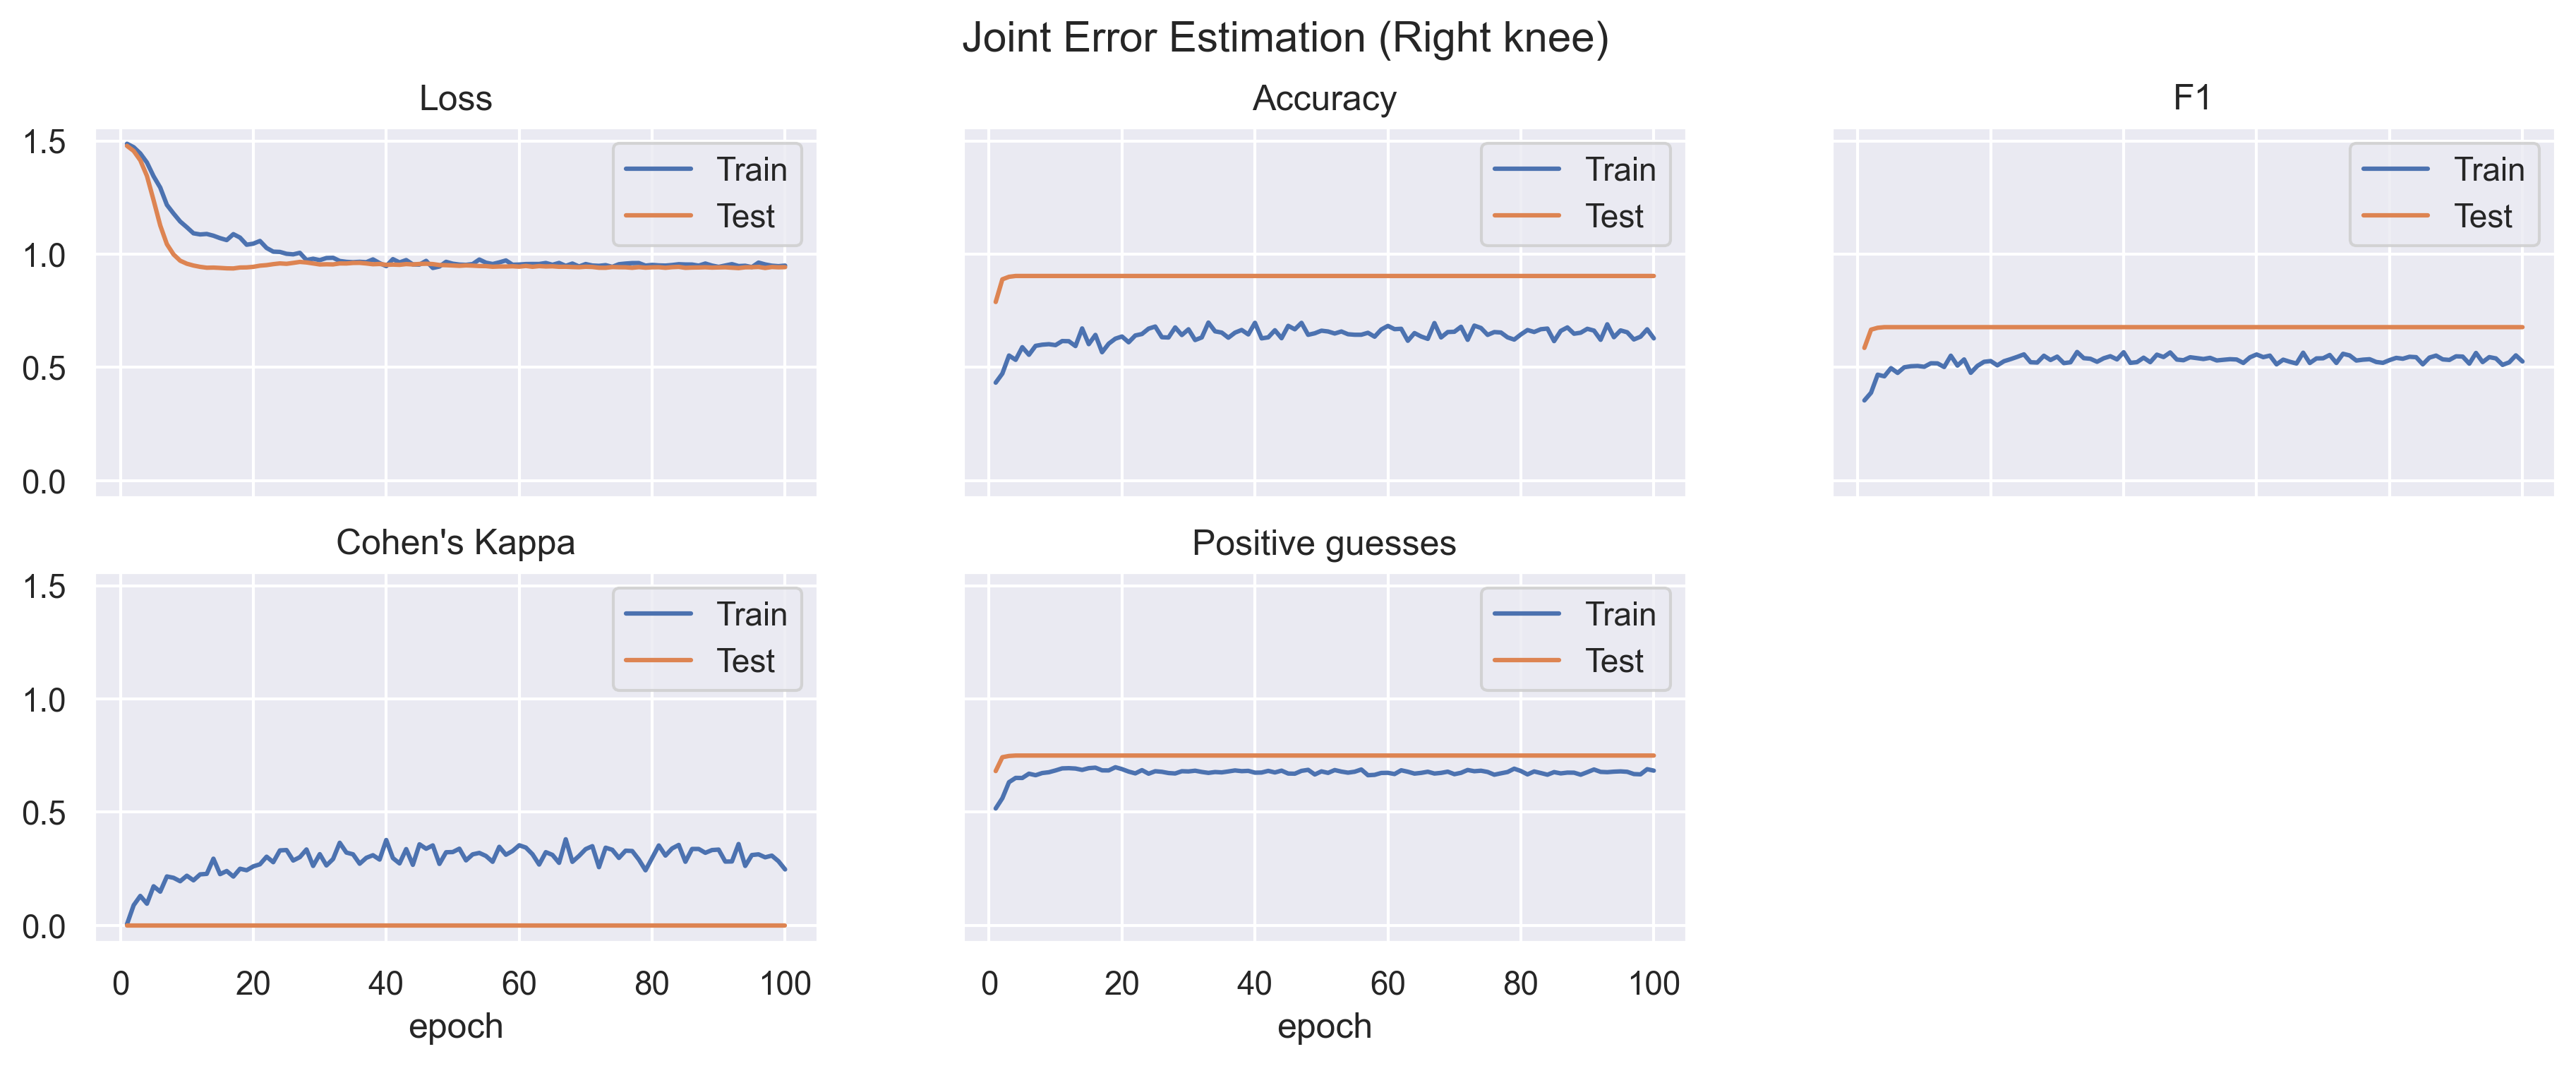
\includegraphics[width=\textwidth]{figures/Results/jt/JointErrorEstimation_Right knee.png}
      \caption{Right Knee Error Estimation}
      \label{fig:rikn_jt_ee}
  \end{subfigure}
  \hfill
  \begin{subfigure}[b]{0.47\linewidth}
      \centering
      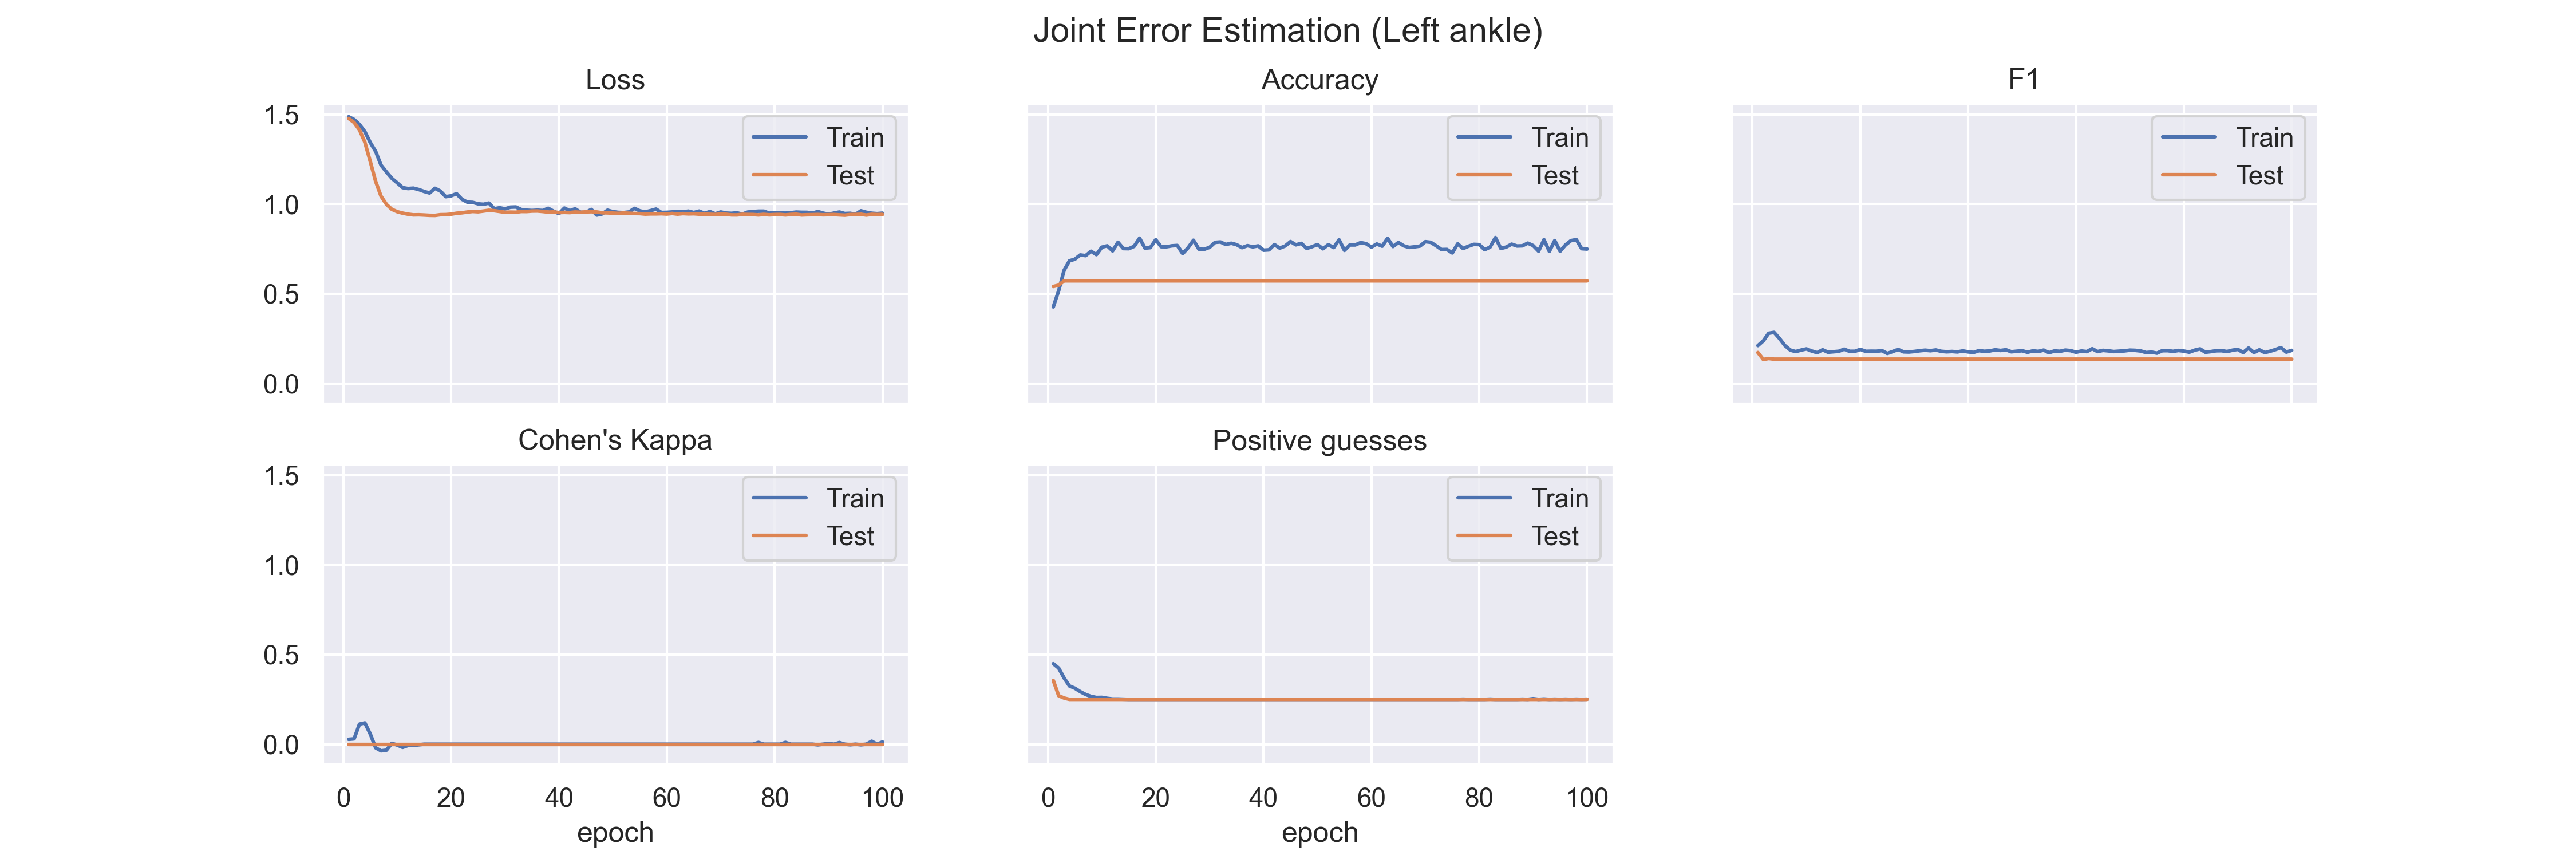
\includegraphics[width=\textwidth]{figures/Results/jt/JointErrorEstimation_Left ankle.png}
      \caption{Left Ankle Error Estimation}
      \label{fig:lean_jt_ee}
  \end{subfigure}
  \hfill
  \begin{subfigure}[b]{0.47\linewidth}
      \centering
      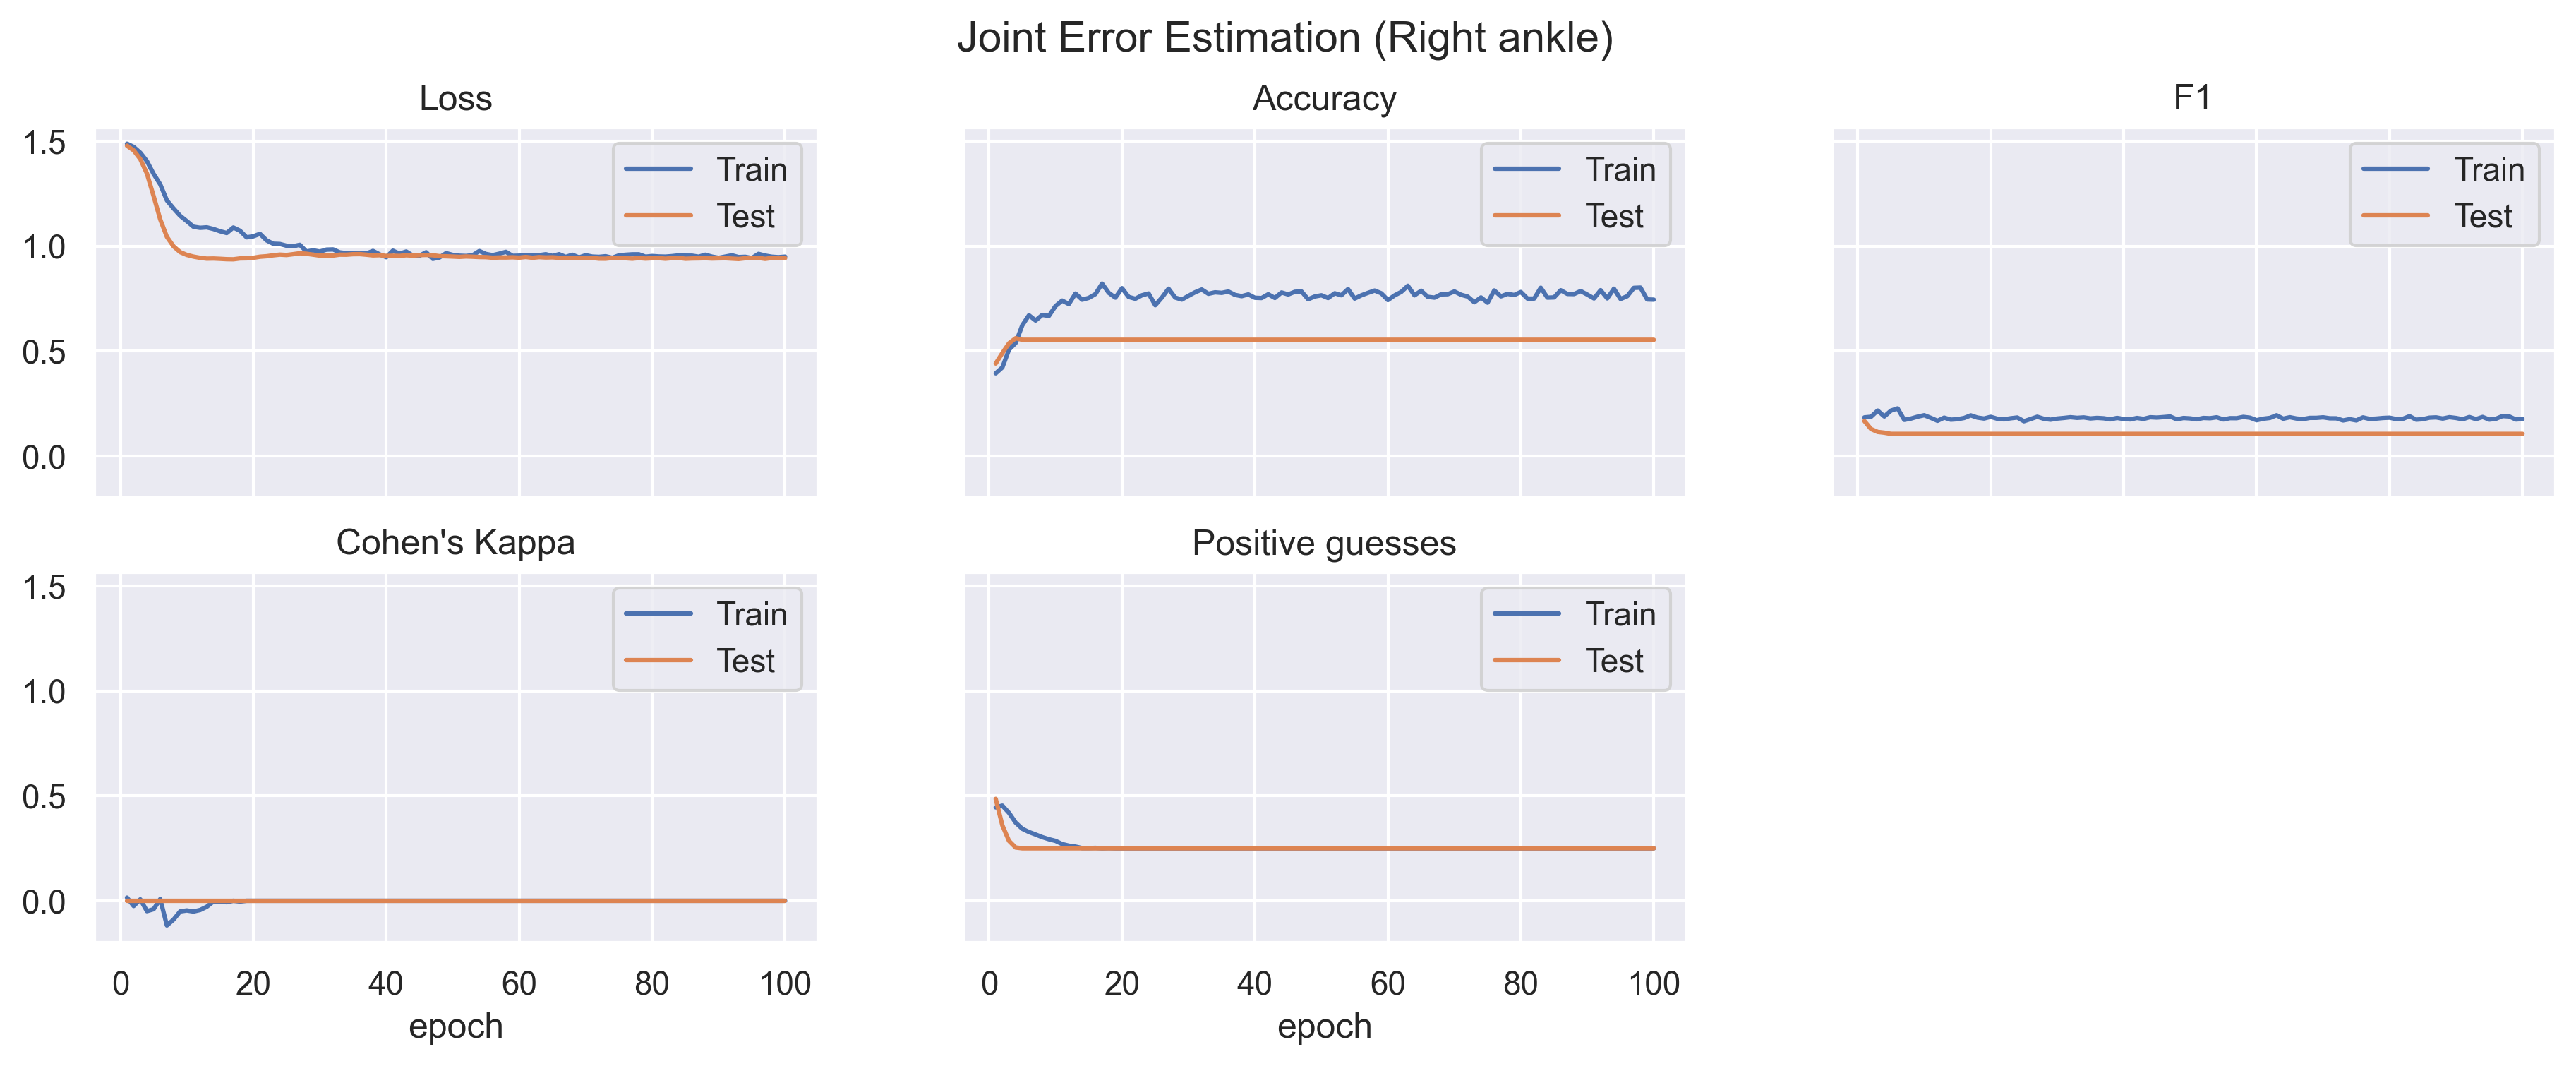
\includegraphics[width=\textwidth]{figures/Results/jt/JointErrorEstimation_Right ankle.png}
      \caption{Right Ankle Error Estimation}
      \label{fig:rian_jt_ee}
  \end{subfigure}
  \caption[Joint model training results]{The training results of the Joint error estimation model. (cont. 4)}
\end{figure}